%%%%%%%% ICML 2023 EXAMPLE LATEX SUBMISSION FILE %%%%%%%%%%%%%%%%%

\documentclass[table]{article}

% Recommended, but optional, packages for figures and better typesetting:
\usepackage{microtype}
\usepackage{graphicx}
\usepackage{subfigure}
\usepackage{booktabs} % for professional tables

% hyperref makes hyperlinks in the resulting PDF.
% If your build breaks (sometimes temporarily if a hyperlink spans a page)
% please comment out the following usepackage line and replace
% \usepackage{icml2023} with \usepackage[nohyperref]{icml2023} above.
\usepackage{hyperref}


% Attempt to make hyperref and algorithmic work together better:
\newcommand{\theHalgorithm}{\arabic{algorithm}}

% Use the following line for the initial blind version submitted for review:
% \usepackage{icml2023}

% If accepted, instead use the following line for the camera-ready submission:
\usepackage[preprint]{icml2025}

% For theorems and such
\usepackage{amsmath}
\usepackage{amssymb}
\usepackage{mathtools}
\usepackage{amsthm}
\usepackage{tikz}
\usepackage{algorithm}
\usepackage{algorithmic}
% if you use cleverer.
\usepackage[capitalize,noabbrev]{cleveref}

%%%%%%%%%%%%%%%%%%%%%%%%%%%%%%%%
% THEOREMS
%%%%%%%%%%%%%%%%%%%%%%%%%%%%%%%%
\theoremstyle{plain}
\newtheorem{theorem}{Theorem}[section]
\newtheorem{proposition}[theorem]{Proposition}
\newtheorem{lemma}[theorem]{Lemma}
\newtheorem{corollary}[theorem]{Corollary}
\newtheorem{fact}[theorem]{Fact}
\theoremstyle{definition}
\newtheorem{definition}[theorem]{Definition}
\newtheorem{assumption}[theorem]{Assumption}
\newtheorem{example}[theorem]{Example}
\newtheorem{remark}[theorem]{Remark}
\newtheorem{note}[theorem]{Note}
\newtheorem{claim}[theorem]{Claim}
\theoremstyle{remark}



% Todonotes is useful during development; simply uncomment the next line
%    and comment out the line below the next line to turn off comments
%\usepackage[disable,textsize=tiny]{todonotes}
\usepackage[textsize=tiny]{todonotes}

%%%%% NEW MATH DEFINITIONS %%%%%

\usepackage{amsmath,amsfonts,bm}
\usepackage{derivative}
% Mark sections of captions for referring to divisions of figures
\newcommand{\figleft}{{\em (Left)}}
\newcommand{\figcenter}{{\em (Center)}}
\newcommand{\figright}{{\em (Right)}}
\newcommand{\figtop}{{\em (Top)}}
\newcommand{\figbottom}{{\em (Bottom)}}
\newcommand{\captiona}{{\em (a)}}
\newcommand{\captionb}{{\em (b)}}
\newcommand{\captionc}{{\em (c)}}
\newcommand{\captiond}{{\em (d)}}

% Highlight a newly defined term
\newcommand{\newterm}[1]{{\bf #1}}

% Derivative d 
\newcommand{\deriv}{{\mathrm{d}}}

% Figure reference, lower-case.
\def\figref#1{figure~\ref{#1}}
% Figure reference, capital. For start of sentence
\def\Figref#1{Figure~\ref{#1}}
\def\twofigref#1#2{figures \ref{#1} and \ref{#2}}
\def\quadfigref#1#2#3#4{figures \ref{#1}, \ref{#2}, \ref{#3} and \ref{#4}}
% Section reference, lower-case.
\def\secref#1{section~\ref{#1}}
% Section reference, capital.
\def\Secref#1{Section~\ref{#1}}
% Reference to two sections.
\def\twosecrefs#1#2{sections \ref{#1} and \ref{#2}}
% Reference to three sections.
\def\secrefs#1#2#3{sections \ref{#1}, \ref{#2} and \ref{#3}}
% Reference to an equation, lower-case.
\def\eqref#1{equation~\ref{#1}}
% Reference to an equation, upper case
\def\Eqref#1{Equation~\ref{#1}}
% A raw reference to an equation---avoid using if possible
\def\plaineqref#1{\ref{#1}}
% Reference to a chapter, lower-case.
\def\chapref#1{chapter~\ref{#1}}
% Reference to an equation, upper case.
\def\Chapref#1{Chapter~\ref{#1}}
% Reference to a range of chapters
\def\rangechapref#1#2{chapters\ref{#1}--\ref{#2}}
% Reference to an algorithm, lower-case.
\def\algref#1{algorithm~\ref{#1}}
% Reference to an algorithm, upper case.
\def\Algref#1{Algorithm~\ref{#1}}
\def\twoalgref#1#2{algorithms \ref{#1} and \ref{#2}}
\def\Twoalgref#1#2{Algorithms \ref{#1} and \ref{#2}}
% Reference to a part, lower case
\def\partref#1{part~\ref{#1}}
% Reference to a part, upper case
\def\Partref#1{Part~\ref{#1}}
\def\twopartref#1#2{parts \ref{#1} and \ref{#2}}

\def\ceil#1{\lceil #1 \rceil}
\def\floor#1{\lfloor #1 \rfloor}
\def\1{\bm{1}}
\newcommand{\train}{\mathcal{D}}
\newcommand{\valid}{\mathcal{D_{\mathrm{valid}}}}
\newcommand{\test}{\mathcal{D_{\mathrm{test}}}}

\def\eps{{\epsilon}}


% Random variables
\def\reta{{\textnormal{$\eta$}}}
\def\ra{{\textnormal{a}}}
\def\rb{{\textnormal{b}}}
\def\rc{{\textnormal{c}}}
\def\rd{{\textnormal{d}}}
\def\re{{\textnormal{e}}}
\def\rf{{\textnormal{f}}}
\def\rg{{\textnormal{g}}}
\def\rh{{\textnormal{h}}}
\def\ri{{\textnormal{i}}}
\def\rj{{\textnormal{j}}}
\def\rk{{\textnormal{k}}}
\def\rl{{\textnormal{l}}}
% rm is already a command, just don't name any random variables m
\def\rn{{\textnormal{n}}}
\def\ro{{\textnormal{o}}}
\def\rp{{\textnormal{p}}}
\def\rq{{\textnormal{q}}}
\def\rr{{\textnormal{r}}}
\def\rs{{\textnormal{s}}}
\def\rt{{\textnormal{t}}}
\def\ru{{\textnormal{u}}}
\def\rv{{\textnormal{v}}}
\def\rw{{\textnormal{w}}}
\def\rx{{\textnormal{x}}}
\def\ry{{\textnormal{y}}}
\def\rz{{\textnormal{z}}}

% Random vectors
\def\rvepsilon{{\mathbf{\epsilon}}}
\def\rvphi{{\mathbf{\phi}}}
\def\rvtheta{{\mathbf{\theta}}}
\def\rva{{\mathbf{a}}}
\def\rvb{{\mathbf{b}}}
\def\rvc{{\mathbf{c}}}
\def\rvd{{\mathbf{d}}}
\def\rve{{\mathbf{e}}}
\def\rvf{{\mathbf{f}}}
\def\rvg{{\mathbf{g}}}
\def\rvh{{\mathbf{h}}}
\def\rvu{{\mathbf{i}}}
\def\rvj{{\mathbf{j}}}
\def\rvk{{\mathbf{k}}}
\def\rvl{{\mathbf{l}}}
\def\rvm{{\mathbf{m}}}
\def\rvn{{\mathbf{n}}}
\def\rvo{{\mathbf{o}}}
\def\rvp{{\mathbf{p}}}
\def\rvq{{\mathbf{q}}}
\def\rvr{{\mathbf{r}}}
\def\rvs{{\mathbf{s}}}
\def\rvt{{\mathbf{t}}}
\def\rvu{{\mathbf{u}}}
\def\rvv{{\mathbf{v}}}
\def\rvw{{\mathbf{w}}}
\def\rvx{{\mathbf{x}}}
\def\rvy{{\mathbf{y}}}
\def\rvz{{\mathbf{z}}}

% Elements of random vectors
\def\erva{{\textnormal{a}}}
\def\ervb{{\textnormal{b}}}
\def\ervc{{\textnormal{c}}}
\def\ervd{{\textnormal{d}}}
\def\erve{{\textnormal{e}}}
\def\ervf{{\textnormal{f}}}
\def\ervg{{\textnormal{g}}}
\def\ervh{{\textnormal{h}}}
\def\ervi{{\textnormal{i}}}
\def\ervj{{\textnormal{j}}}
\def\ervk{{\textnormal{k}}}
\def\ervl{{\textnormal{l}}}
\def\ervm{{\textnormal{m}}}
\def\ervn{{\textnormal{n}}}
\def\ervo{{\textnormal{o}}}
\def\ervp{{\textnormal{p}}}
\def\ervq{{\textnormal{q}}}
\def\ervr{{\textnormal{r}}}
\def\ervs{{\textnormal{s}}}
\def\ervt{{\textnormal{t}}}
\def\ervu{{\textnormal{u}}}
\def\ervv{{\textnormal{v}}}
\def\ervw{{\textnormal{w}}}
\def\ervx{{\textnormal{x}}}
\def\ervy{{\textnormal{y}}}
\def\ervz{{\textnormal{z}}}

% Random matrices
\def\rmA{{\mathbf{A}}}
\def\rmB{{\mathbf{B}}}
\def\rmC{{\mathbf{C}}}
\def\rmD{{\mathbf{D}}}
\def\rmE{{\mathbf{E}}}
\def\rmF{{\mathbf{F}}}
\def\rmG{{\mathbf{G}}}
\def\rmH{{\mathbf{H}}}
\def\rmI{{\mathbf{I}}}
\def\rmJ{{\mathbf{J}}}
\def\rmK{{\mathbf{K}}}
\def\rmL{{\mathbf{L}}}
\def\rmM{{\mathbf{M}}}
\def\rmN{{\mathbf{N}}}
\def\rmO{{\mathbf{O}}}
\def\rmP{{\mathbf{P}}}
\def\rmQ{{\mathbf{Q}}}
\def\rmR{{\mathbf{R}}}
\def\rmS{{\mathbf{S}}}
\def\rmT{{\mathbf{T}}}
\def\rmU{{\mathbf{U}}}
\def\rmV{{\mathbf{V}}}
\def\rmW{{\mathbf{W}}}
\def\rmX{{\mathbf{X}}}
\def\rmY{{\mathbf{Y}}}
\def\rmZ{{\mathbf{Z}}}

% Elements of random matrices
\def\ermA{{\textnormal{A}}}
\def\ermB{{\textnormal{B}}}
\def\ermC{{\textnormal{C}}}
\def\ermD{{\textnormal{D}}}
\def\ermE{{\textnormal{E}}}
\def\ermF{{\textnormal{F}}}
\def\ermG{{\textnormal{G}}}
\def\ermH{{\textnormal{H}}}
\def\ermI{{\textnormal{I}}}
\def\ermJ{{\textnormal{J}}}
\def\ermK{{\textnormal{K}}}
\def\ermL{{\textnormal{L}}}
\def\ermM{{\textnormal{M}}}
\def\ermN{{\textnormal{N}}}
\def\ermO{{\textnormal{O}}}
\def\ermP{{\textnormal{P}}}
\def\ermQ{{\textnormal{Q}}}
\def\ermR{{\textnormal{R}}}
\def\ermS{{\textnormal{S}}}
\def\ermT{{\textnormal{T}}}
\def\ermU{{\textnormal{U}}}
\def\ermV{{\textnormal{V}}}
\def\ermW{{\textnormal{W}}}
\def\ermX{{\textnormal{X}}}
\def\ermY{{\textnormal{Y}}}
\def\ermZ{{\textnormal{Z}}}

% Vectors
\def\vzero{{\bm{0}}}
\def\vone{{\bm{1}}}
\def\vmu{{\bm{\mu}}}
\def\vtheta{{\bm{\theta}}}
\def\vphi{{\bm{\phi}}}
\def\va{{\bm{a}}}
\def\vb{{\bm{b}}}
\def\vc{{\bm{c}}}
\def\vd{{\bm{d}}}
\def\ve{{\bm{e}}}
\def\vf{{\bm{f}}}
\def\vg{{\bm{g}}}
\def\vh{{\bm{h}}}
\def\vi{{\bm{i}}}
\def\vj{{\bm{j}}}
\def\vk{{\bm{k}}}
\def\vl{{\bm{l}}}
\def\vm{{\bm{m}}}
\def\vn{{\bm{n}}}
\def\vo{{\bm{o}}}
\def\vp{{\bm{p}}}
\def\vq{{\bm{q}}}
\def\vr{{\bm{r}}}
\def\vs{{\bm{s}}}
\def\vt{{\bm{t}}}
\def\vu{{\bm{u}}}
\def\vv{{\bm{v}}}
\def\vw{{\bm{w}}}
\def\vx{{\bm{x}}}
\def\vy{{\bm{y}}}
\def\vz{{\bm{z}}}

% Elements of vectors
\def\evalpha{{\alpha}}
\def\evbeta{{\beta}}
\def\evepsilon{{\epsilon}}
\def\evlambda{{\lambda}}
\def\evomega{{\omega}}
\def\evmu{{\mu}}
\def\evpsi{{\psi}}
\def\evsigma{{\sigma}}
\def\evtheta{{\theta}}
\def\eva{{a}}
\def\evb{{b}}
\def\evc{{c}}
\def\evd{{d}}
\def\eve{{e}}
\def\evf{{f}}
\def\evg{{g}}
\def\evh{{h}}
\def\evi{{i}}
\def\evj{{j}}
\def\evk{{k}}
\def\evl{{l}}
\def\evm{{m}}
\def\evn{{n}}
\def\evo{{o}}
\def\evp{{p}}
\def\evq{{q}}
\def\evr{{r}}
\def\evs{{s}}
\def\evt{{t}}
\def\evu{{u}}
\def\evv{{v}}
\def\evw{{w}}
\def\evx{{x}}
\def\evy{{y}}
\def\evz{{z}}

% Matrix
\def\mA{{\bm{A}}}
\def\mB{{\bm{B}}}
\def\mC{{\bm{C}}}
\def\mD{{\bm{D}}}
\def\mE{{\bm{E}}}
\def\mF{{\bm{F}}}
\def\mG{{\bm{G}}}
\def\mH{{\bm{H}}}
\def\mI{{\bm{I}}}
\def\mJ{{\bm{J}}}
\def\mK{{\bm{K}}}
\def\mL{{\bm{L}}}
\def\mM{{\bm{M}}}
\def\mN{{\bm{N}}}
\def\mO{{\bm{O}}}
\def\mP{{\bm{P}}}
\def\mQ{{\bm{Q}}}
\def\mR{{\bm{R}}}
\def\mS{{\bm{S}}}
\def\mT{{\bm{T}}}
\def\mU{{\bm{U}}}
\def\mV{{\bm{V}}}
\def\mW{{\bm{W}}}
\def\mX{{\bm{X}}}
\def\mY{{\bm{Y}}}
\def\mZ{{\bm{Z}}}
\def\mBeta{{\bm{\beta}}}
\def\mPhi{{\bm{\Phi}}}
\def\mLambda{{\bm{\Lambda}}}
\def\mSigma{{\bm{\Sigma}}}

% Tensor
\DeclareMathAlphabet{\mathsfit}{\encodingdefault}{\sfdefault}{m}{sl}
\SetMathAlphabet{\mathsfit}{bold}{\encodingdefault}{\sfdefault}{bx}{n}
\newcommand{\tens}[1]{\bm{\mathsfit{#1}}}
\def\tA{{\tens{A}}}
\def\tB{{\tens{B}}}
\def\tC{{\tens{C}}}
\def\tD{{\tens{D}}}
\def\tE{{\tens{E}}}
\def\tF{{\tens{F}}}
\def\tG{{\tens{G}}}
\def\tH{{\tens{H}}}
\def\tI{{\tens{I}}}
\def\tJ{{\tens{J}}}
\def\tK{{\tens{K}}}
\def\tL{{\tens{L}}}
\def\tM{{\tens{M}}}
\def\tN{{\tens{N}}}
\def\tO{{\tens{O}}}
\def\tP{{\tens{P}}}
\def\tQ{{\tens{Q}}}
\def\tR{{\tens{R}}}
\def\tS{{\tens{S}}}
\def\tT{{\tens{T}}}
\def\tU{{\tens{U}}}
\def\tV{{\tens{V}}}
\def\tW{{\tens{W}}}
\def\tX{{\tens{X}}}
\def\tY{{\tens{Y}}}
\def\tZ{{\tens{Z}}}


% Graph
\def\gA{{\mathcal{A}}}
\def\gB{{\mathcal{B}}}
\def\gC{{\mathcal{C}}}
\def\gD{{\mathcal{D}}}
\def\gE{{\mathcal{E}}}
\def\gF{{\mathcal{F}}}
\def\gG{{\mathcal{G}}}
\def\gH{{\mathcal{H}}}
\def\gI{{\mathcal{I}}}
\def\gJ{{\mathcal{J}}}
\def\gK{{\mathcal{K}}}
\def\gL{{\mathcal{L}}}
\def\gM{{\mathcal{M}}}
\def\gN{{\mathcal{N}}}
\def\gO{{\mathcal{O}}}
\def\gP{{\mathcal{P}}}
\def\gQ{{\mathcal{Q}}}
\def\gR{{\mathcal{R}}}
\def\gS{{\mathcal{S}}}
\def\gT{{\mathcal{T}}}
\def\gU{{\mathcal{U}}}
\def\gV{{\mathcal{V}}}
\def\gW{{\mathcal{W}}}
\def\gX{{\mathcal{X}}}
\def\gY{{\mathcal{Y}}}
\def\gZ{{\mathcal{Z}}}

% Sets
\def\sA{{\mathbb{A}}}
\def\sB{{\mathbb{B}}}
\def\sC{{\mathbb{C}}}
\def\sD{{\mathbb{D}}}
% Don't use a set called E, because this would be the same as our symbol
% for expectation.
\def\sF{{\mathbb{F}}}
\def\sG{{\mathbb{G}}}
\def\sH{{\mathbb{H}}}
\def\sI{{\mathbb{I}}}
\def\sJ{{\mathbb{J}}}
\def\sK{{\mathbb{K}}}
\def\sL{{\mathbb{L}}}
\def\sM{{\mathbb{M}}}
\def\sN{{\mathbb{N}}}
\def\sO{{\mathbb{O}}}
\def\sP{{\mathbb{P}}}
\def\sQ{{\mathbb{Q}}}
\def\sR{{\mathbb{R}}}
\def\sS{{\mathbb{S}}}
\def\sT{{\mathbb{T}}}
\def\sU{{\mathbb{U}}}
\def\sV{{\mathbb{V}}}
\def\sW{{\mathbb{W}}}
\def\sX{{\mathbb{X}}}
\def\sY{{\mathbb{Y}}}
\def\sZ{{\mathbb{Z}}}

% Entries of a matrix
\def\emLambda{{\Lambda}}
\def\emA{{A}}
\def\emB{{B}}
\def\emC{{C}}
\def\emD{{D}}
\def\emE{{E}}
\def\emF{{F}}
\def\emG{{G}}
\def\emH{{H}}
\def\emI{{I}}
\def\emJ{{J}}
\def\emK{{K}}
\def\emL{{L}}
\def\emM{{M}}
\def\emN{{N}}
\def\emO{{O}}
\def\emP{{P}}
\def\emQ{{Q}}
\def\emR{{R}}
\def\emS{{S}}
\def\emT{{T}}
\def\emU{{U}}
\def\emV{{V}}
\def\emW{{W}}
\def\emX{{X}}
\def\emY{{Y}}
\def\emZ{{Z}}
\def\emSigma{{\Sigma}}

% entries of a tensor
% Same font as tensor, without \bm wrapper
\newcommand{\etens}[1]{\mathsfit{#1}}
\def\etLambda{{\etens{\Lambda}}}
\def\etA{{\etens{A}}}
\def\etB{{\etens{B}}}
\def\etC{{\etens{C}}}
\def\etD{{\etens{D}}}
\def\etE{{\etens{E}}}
\def\etF{{\etens{F}}}
\def\etG{{\etens{G}}}
\def\etH{{\etens{H}}}
\def\etI{{\etens{I}}}
\def\etJ{{\etens{J}}}
\def\etK{{\etens{K}}}
\def\etL{{\etens{L}}}
\def\etM{{\etens{M}}}
\def\etN{{\etens{N}}}
\def\etO{{\etens{O}}}
\def\etP{{\etens{P}}}
\def\etQ{{\etens{Q}}}
\def\etR{{\etens{R}}}
\def\etS{{\etens{S}}}
\def\etT{{\etens{T}}}
\def\etU{{\etens{U}}}
\def\etV{{\etens{V}}}
\def\etW{{\etens{W}}}
\def\etX{{\etens{X}}}
\def\etY{{\etens{Y}}}
\def\etZ{{\etens{Z}}}

% The true underlying data generating distribution
\newcommand{\pdata}{p_{\rm{data}}}
\newcommand{\ptarget}{p_{\rm{target}}}
\newcommand{\pprior}{p_{\rm{prior}}}
\newcommand{\pbase}{p_{\rm{base}}}
\newcommand{\pref}{p_{\rm{ref}}}

% The empirical distribution defined by the training set
\newcommand{\ptrain}{\hat{p}_{\rm{data}}}
\newcommand{\Ptrain}{\hat{P}_{\rm{data}}}
% The model distribution
\newcommand{\pmodel}{p_{\rm{model}}}
\newcommand{\Pmodel}{P_{\rm{model}}}
\newcommand{\ptildemodel}{\tilde{p}_{\rm{model}}}
% Stochastic autoencoder distributions
\newcommand{\pencode}{p_{\rm{encoder}}}
\newcommand{\pdecode}{p_{\rm{decoder}}}
\newcommand{\precons}{p_{\rm{reconstruct}}}

\newcommand{\laplace}{\mathrm{Laplace}} % Laplace distribution

\newcommand{\E}{\mathbb{E}}
\newcommand{\Ls}{\mathcal{L}}
\newcommand{\R}{\mathbb{R}}
\newcommand{\emp}{\tilde{p}}
\newcommand{\lr}{\alpha}
\newcommand{\reg}{\lambda}
\newcommand{\rect}{\mathrm{rectifier}}
\newcommand{\softmax}{\mathrm{softmax}}
\newcommand{\sigmoid}{\sigma}
\newcommand{\softplus}{\zeta}
\newcommand{\KL}{D_{\mathrm{KL}}}
\newcommand{\Var}{\mathrm{Var}}
\newcommand{\standarderror}{\mathrm{SE}}
\newcommand{\Cov}{\mathrm{Cov}}
% Wolfram Mathworld says $L^2$ is for function spaces and $\ell^2$ is for vectors
% But then they seem to use $L^2$ for vectors throughout the site, and so does
% wikipedia.
\newcommand{\normlzero}{L^0}
\newcommand{\normlone}{L^1}
\newcommand{\normltwo}{L^2}
\newcommand{\normlp}{L^p}
\newcommand{\normmax}{L^\infty}

\newcommand{\parents}{Pa} % See usage in notation.tex. Chosen to match Daphne's book.

\DeclareMathOperator*{\argmax}{arg\,max}
\DeclareMathOperator*{\argmin}{arg\,min}

\DeclareMathOperator{\sign}{sign}
\DeclareMathOperator{\Tr}{Tr}
\let\ab\allowbreak

\newcommand*{\ldblbrace}{\{\mskip-5mu\{}
\newcommand*{\rdblbrace}{\}\mskip-5mu\}}
\newcommand*{\Ldblbrace}{\left\{\mskip-7mu\left\{}
\newcommand*{\Rdblbrace}{\right\}\mskip-7mu\right\}}
\newcommand*{\dis}{{\operatorname{dis}}}
\newcommand*{\disR}{\operatorname{dis}^\mathsf{R}}
\newcommand*{\disH}{\operatorname{dis}^\mathsf{H}}
\newcommand*{\hash}{\mathsf{hash}}
\newcommand*{\op}{\mathsf{op}}
\newcommand*{\agg}{\mathsf{agg}}
\newcommand*{\walk}{\mathsf{walk}}
\newcommand*{\pool}{\mathsf{Pool}}
\newcommand*{\twist}{\mathsf{twist}}
\newcommand*{\meta}{\mathsf{Meta}}
\newcommand*{\DKL}[2]{\KL(#1\|#2)}
\newcommand*{\DEP}{\operatorname{DEP}}
\newcommand*{\SEP}{\operatorname{SEP}}
\newcommand*{\NEW}{\operatorname{NEW}}
\newcommand*{\PPL}{\operatorname{TER}}
\newcommand*{\SER}{\operatorname{SER}}
\newcommand*{\PROC}{\operatorname{REVR}}
\newcommand*{\mask}{\texttt{[m]}}
\newcommand*{\MK}[1]{\textcolor{red}{[Mark: #1]}}
\newcommand*{\guhao}[1]{\textcolor{blue}{[guhao: #1]}}
\newcommand*{\yihan}[1]{\textcolor{purple}{[yihan: #1]}}
\newcommand{\TO}{\textbf{ to }}
\newcommand{\RETURN}{\STATE \textbf{return} }
\usepackage{enumitem}
\usepackage{makecell}
\usepackage{multirow}
\usepackage{mathrsfs}
% \usepackage[table]{xcolor}

% The \icmltitle you define below is probably too long as a header.
% Therefore, a short form for the running title is supplied here:
\icmltitlerunning{Theoretical Benefit and Limitation of Diffusion Language Model}

\begin{document}

\twocolumn[
\icmltitle{Theoretical Benefit and Limitation of Diffusion Language Model}

% It is OKAY to include author information, even for blind
% submissions: the style file will automatically remove it for you
% unless you've provided the [accepted] option to the icml2023
% package.

% List of affiliations: The first argument should be a (short)
% identifier you will use later to specify author affiliations
% Academic affiliations should list Department, University, City, Region, Country
% Industry affiliations should list Company, City, Region, Country

% You can specify symbols, otherwise they are numbered in order.
% Ideally, you should not use this facility. Affiliations will be numbered
% in order of appearance and this is the preferred way.
\icmlsetsymbol{equal}{*}

\vspace{-3pt}
\begin{icmlauthorlist}
\icmlauthor{Guhao Feng}{equal,pku}
\icmlauthor{Yihan Geng}{equal,pku}
\icmlauthor{Jian Guan}{ant}
\icmlauthor{Wei Wu}{ant}
\icmlauthor{Liwei Wang}{pku}
\icmlauthor{Di He}{pku}
\end{icmlauthorlist}
\icmlaffiliation{pku}{Peking University}
\icmlaffiliation{ant}{Ant Group}
% \icmlaffiliation{pku1}{National Key Laboratory of General Artificial Intelligence, School of Intelligence Science and Technology, Peking University}
% \icmlaffiliation{pku2}{Center for Data Science, Peking University}
% \icmlaffiliation{pku3}{School of Mathematical Sciences, Peking University}

% \icmlcorrespondingauthor{Guhao Feng}{fenguhao@stu.pku.edu.cn}
% \icmlcorrespondingauthor{Liwei Wang}{wanglw@cis.pku.edu.cn}
% \icmlcorrespondingauthor{Di He}{dihe@pku.edu.cn}


% You may provide any keywords that you
% find helpful for describing your paper; these are used to populate
% the "keywords" metadata in the PDF but will not be shown in the document
\icmlkeywords{Machine Learning, ICML}

\vskip 0.24in
]

% this must go after the closing bracket ] following \twocolumn[ ...

% This command actually creates the footnote in the first column
% listing the affiliations and the copyright notice.
% The command takes one argument, which is text to display at the start of the footnote.
% The \icmlEqualContribution command is standard text for equal contribution.
% Remove it (just {}) if you do not need this facility.

%\printAffiliationsAndNotice{}  % leave blank if no need to mention equal contribution
\printAffiliationsAndNotice{\icmlEqualContribution} % otherwise use the standard text.

\begin{abstract}
Diffusion language models have emerged as a promising approach for text generation. One would naturally expect this method to be an efficient replacement for autoregressive models since multiple tokens can be sampled in parallel during each diffusion step. However, its efficiency-accuracy trade-off is not yet well understood. In this paper, we present a rigorous theoretical analysis of a widely used type of diffusion language model, the Masked Diffusion Model (MDM), and find that its effectiveness heavily depends on the target evaluation metric. Under mild conditions, we prove that when using perplexity as the metric, MDMs can achieve near-optimal perplexity in sampling steps regardless of sequence length, demonstrating that efficiency can be achieved without sacrificing performance. However, when using the sequence error rate--which is important for understanding the ``correctness" of a sequence, such as a reasoning chain--we show that the required sampling steps must scale linearly with sequence length to obtain ``correct" sequences, thereby eliminating MDM's efficiency advantage over autoregressive models. Our analysis establishes the first theoretical foundation for understanding the benefits and limitations of MDMs. All theoretical findings are supported by empirical studies.
\end{abstract}

\section{Introduction}

Large language models (LLMs) have achieved remarkable success in automated math problem solving, particularly through code-generation capabilities integrated with proof assistants~\citep{lean,isabelle,POT,autoformalization,MATH}. Although LLMs excel at generating solution steps and correct answers in algebra and calculus~\citep{math_solving}, their unimodal nature limits performance in plane geometry, where solution depends on both diagram and text~\citep{math_solving}. 

Specialized vision-language models (VLMs) have accordingly been developed for plane geometry problem solving (PGPS)~\citep{geoqa,unigeo,intergps,pgps,GOLD,LANS,geox}. Yet, it remains unclear whether these models genuinely leverage diagrams or rely almost exclusively on textual features. This ambiguity arises because existing PGPS datasets typically embed sufficient geometric details within problem statements, potentially making the vision encoder unnecessary~\citep{GOLD}. \cref{fig:pgps_examples} illustrates example questions from GeoQA and PGPS9K, where solutions can be derived without referencing the diagrams.

\begin{figure}
    \centering
    \begin{subfigure}[t]{.49\linewidth}
        \centering
        \includegraphics[width=\linewidth]{latex/figures/images/geoqa_example.pdf}
        \caption{GeoQA}
        \label{fig:geoqa_example}
    \end{subfigure}
    \begin{subfigure}[t]{.48\linewidth}
        \centering
        \includegraphics[width=\linewidth]{latex/figures/images/pgps_example.pdf}
        \caption{PGPS9K}
        \label{fig:pgps9k_example}
    \end{subfigure}
    \caption{
    Examples of diagram-caption pairs and their solution steps written in formal languages from GeoQA and PGPS9k datasets. In the problem description, the visual geometric premises and numerical variables are highlighted in green and red, respectively. A significant difference in the style of the diagram and formal language can be observable. %, along with the differences in formal languages supported by the corresponding datasets.
    \label{fig:pgps_examples}
    }
\end{figure}



We propose a new benchmark created via a synthetic data engine, which systematically evaluates the ability of VLM vision encoders to recognize geometric premises. Our empirical findings reveal that previously suggested self-supervised learning (SSL) approaches, e.g., vector quantized variataional auto-encoder (VQ-VAE)~\citep{unimath} and masked auto-encoder (MAE)~\citep{scagps,geox}, and widely adopted encoders, e.g., OpenCLIP~\citep{clip} and DinoV2~\citep{dinov2}, struggle to detect geometric features such as perpendicularity and degrees. 

To this end, we propose \geoclip{}, a model pre-trained on a large corpus of synthetic diagram–caption pairs. By varying diagram styles (e.g., color, font size, resolution, line width), \geoclip{} learns robust geometric representations and outperforms prior SSL-based methods on our benchmark. Building on \geoclip{}, we introduce a few-shot domain adaptation technique that efficiently transfers the recognition ability to real-world diagrams. We further combine this domain-adapted GeoCLIP with an LLM, forming a domain-agnostic VLM for solving PGPS tasks in MathVerse~\citep{mathverse}. 
%To accommodate diverse diagram styles and solution formats, we unify the solution program languages across multiple PGPS datasets, ensuring comprehensive evaluation. 

In our experiments on MathVerse~\citep{mathverse}, which encompasses diverse plane geometry tasks and diagram styles, our VLM with a domain-adapted \geoclip{} consistently outperforms both task-specific PGPS models and generalist VLMs. 
% In particular, it achieves higher accuracy on tasks requiring geometric-feature recognition, even when critical numerical measurements are moved from text to diagrams. 
Ablation studies confirm the effectiveness of our domain adaptation strategy, showing improvements in optical character recognition (OCR)-based tasks and robust diagram embeddings across different styles. 
% By unifying the solution program languages of existing datasets and incorporating OCR capability, we enable a single VLM, named \geovlm{}, to handle a broad class of plane geometry problems.

% Contributions
We summarize the contributions as follows:
We propose a novel benchmark for systematically assessing how well vision encoders recognize geometric premises in plane geometry diagrams~(\cref{sec:visual_feature}); We introduce \geoclip{}, a vision encoder capable of accurately detecting visual geometric premises~(\cref{sec:geoclip}), and a few-shot domain adaptation technique that efficiently transfers this capability across different diagram styles (\cref{sec:domain_adaptation});
We show that our VLM, incorporating domain-adapted GeoCLIP, surpasses existing specialized PGPS VLMs and generalist VLMs on the MathVerse benchmark~(\cref{sec:experiments}) and effectively interprets diverse diagram styles~(\cref{sec:abl}).

\iffalse
\begin{itemize}
    \item We propose a novel benchmark for systematically assessing how well vision encoders recognize geometric premises, e.g., perpendicularity and angle measures, in plane geometry diagrams.
	\item We introduce \geoclip{}, a vision encoder capable of accurately detecting visual geometric premises, and a few-shot domain adaptation technique that efficiently transfers this capability across different diagram styles.
	\item We show that our final VLM, incorporating GeoCLIP-DA, effectively interprets diverse diagram styles and achieves state-of-the-art performance on the MathVerse benchmark, surpassing existing specialized PGPS models and generalist VLM models.
\end{itemize}
\fi

\iffalse

Large language models (LLMs) have made significant strides in automated math word problem solving. In particular, their code-generation capabilities combined with proof assistants~\citep{lean,isabelle} help minimize computational errors~\citep{POT}, improve solution precision~\citep{autoformalization}, and offer rigorous feedback and evaluation~\citep{MATH}. Although LLMs excel in generating solution steps and correct answers for algebra and calculus~\citep{math_solving}, their uni-modal nature limits performance in domains like plane geometry, where both diagrams and text are vital.

Plane geometry problem solving (PGPS) tasks typically include diagrams and textual descriptions, requiring solvers to interpret premises from both sources. To facilitate automated solutions for these problems, several studies have introduced formal languages tailored for plane geometry to represent solution steps as a program with training datasets composed of diagrams, textual descriptions, and solution programs~\citep{geoqa,unigeo,intergps,pgps}. Building on these datasets, a number of PGPS specialized vision-language models (VLMs) have been developed so far~\citep{GOLD, LANS, geox}.

Most existing VLMs, however, fail to use diagrams when solving geometry problems. Well-known PGPS datasets such as GeoQA~\citep{geoqa}, UniGeo~\citep{unigeo}, and PGPS9K~\citep{pgps}, can be solved without accessing diagrams, as their problem descriptions often contain all geometric information. \cref{fig:pgps_examples} shows an example from GeoQA and PGPS9K datasets, where one can deduce the solution steps without knowing the diagrams. 
As a result, models trained on these datasets rely almost exclusively on textual information, leaving the vision encoder under-utilized~\citep{GOLD}. 
Consequently, the VLMs trained on these datasets cannot solve the plane geometry problem when necessary geometric properties or relations are excluded from the problem statement.

Some studies seek to enhance the recognition of geometric premises from a diagram by directly predicting the premises from the diagram~\citep{GOLD, intergps} or as an auxiliary task for vision encoders~\citep{geoqa,geoqa-plus}. However, these approaches remain highly domain-specific because the labels for training are difficult to obtain, thus limiting generalization across different domains. While self-supervised learning (SSL) methods that depend exclusively on geometric diagrams, e.g., vector quantized variational auto-encoder (VQ-VAE)~\citep{unimath} and masked auto-encoder (MAE)~\citep{scagps,geox}, have also been explored, the effectiveness of the SSL approaches on recognizing geometric features has not been thoroughly investigated.

We introduce a benchmark constructed with a synthetic data engine to evaluate the effectiveness of SSL approaches in recognizing geometric premises from diagrams. Our empirical results with the proposed benchmark show that the vision encoders trained with SSL methods fail to capture visual \geofeat{}s such as perpendicularity between two lines and angle measure.
Furthermore, we find that the pre-trained vision encoders often used in general-purpose VLMs, e.g., OpenCLIP~\citep{clip} and DinoV2~\citep{dinov2}, fail to recognize geometric premises from diagrams.

To improve the vision encoder for PGPS, we propose \geoclip{}, a model trained with a massive amount of diagram-caption pairs.
Since the amount of diagram-caption pairs in existing benchmarks is often limited, we develop a plane diagram generator that can randomly sample plane geometry problems with the help of existing proof assistant~\citep{alphageometry}.
To make \geoclip{} robust against different styles, we vary the visual properties of diagrams, such as color, font size, resolution, and line width.
We show that \geoclip{} performs better than the other SSL approaches and commonly used vision encoders on the newly proposed benchmark.

Another major challenge in PGPS is developing a domain-agnostic VLM capable of handling multiple PGPS benchmarks. As shown in \cref{fig:pgps_examples}, the main difficulties arise from variations in diagram styles. 
To address the issue, we propose a few-shot domain adaptation technique for \geoclip{} which transfers its visual \geofeat{} perception from the synthetic diagrams to the real-world diagrams efficiently. 

We study the efficacy of the domain adapted \geoclip{} on PGPS when equipped with the language model. To be specific, we compare the VLM with the previous PGPS models on MathVerse~\citep{mathverse}, which is designed to evaluate both the PGPS and visual \geofeat{} perception performance on various domains.
While previous PGPS models are inapplicable to certain types of MathVerse problems, we modify the prediction target and unify the solution program languages of the existing PGPS training data to make our VLM applicable to all types of MathVerse problems.
Results on MathVerse demonstrate that our VLM more effectively integrates diagrammatic information and remains robust under conditions of various diagram styles.

\begin{itemize}
    \item We propose a benchmark to measure the visual \geofeat{} recognition performance of different vision encoders.
    % \item \sh{We introduce geometric CLIP (\geoclip{} and train the VLM equipped with \geoclip{} to predict both solution steps and the numerical measurements of the problem.}
    \item We introduce \geoclip{}, a vision encoder which can accurately recognize visual \geofeat{}s and a few-shot domain adaptation technique which can transfer such ability to different domains efficiently. 
    % \item \sh{We develop our final PGPS model, \geovlm{}, by adapting \geoclip{} to different domains and training with unified languages of solution program data.}
    % We develop a domain-agnostic VLM, namely \geovlm{}, by applying a simple yet effective domain adaptation method to \geoclip{} and training on the refined training data.
    \item We demonstrate our VLM equipped with GeoCLIP-DA effectively interprets diverse diagram styles, achieving superior performance on MathVerse compared to the existing PGPS models.
\end{itemize}

\fi 

\section{Preliminaries}
\label{Preliminaries}
\subsection{Multi-Agent Reinforcement Learning}
A MARL problem can be formulated as a decentralized partially observed Markov decision process (Dec-POMDP)~\cite{oliehoek2016concise}, which is described as a tuple $\langle n,\boldsymbol{S},\boldsymbol{A},P,R,\boldsymbol{O},\boldsymbol{\Omega},\gamma\rangle $, where $n$ represents the number of agents, $\boldsymbol{S}$ is the global state space. $\boldsymbol{A}$ is the action space. $\boldsymbol{O}=\{O_{i}\}_{i=1,\cdots,n}$ is the observation space. At timestep $t$, each agent $i$ receives an observation $o_{i}^t\in O_{i}$ according to the observation function $\boldsymbol{\Omega}(s^t,i):\boldsymbol{S}\to O_i$ and then selects an action $a_i^t\in\boldsymbol{A}$. The joint action $\boldsymbol{a}^t=(a_1^t,\ldots,a_n^t)$ is then applied to the environment, resulting in a transition to the next state $s^{t+1}$ and a global reward signal $r^{t}$ according to the transition function $P(s^{t+1}\mid s^{t},\boldsymbol{a}^t)$ and the reward function $R(s^t,\boldsymbol{a}^t)$. $\gamma\in[0,1]$ is the discount factor. The objective is to learn a joint policy $\pi$ that maximizes the expected cumulative reward $\mathbb{E}\left[\sum_{t=0}^{\infty}\gamma^{t}r^{t}\right|\pi]$.

\subsection{Centralized Training With Decentralized Execution}
Centralized Training with Decentralized Execution (CTDE) is a commonly employed architecture in MARL~\cite{lowe2017multi,rashid2020monotonic}. In CTDE, each agent utilizes an actor network to make decisions based on local observations. Additionally, the training process incorporates global information to train a centralized value function. The centralized value function provides a centralized gradient to update the actor network based on its outputs.

\subsection{Generalizable Model Structure in MARL}
To handle varying state/observation/action spaces, previous works like UPDeT~\cite{hu2021updet} and ASN~\cite{wang2019action} propose a generalizable model that treats all agents as entities. In such models, observation $o_i$ can be conducted as entity-observations: $[o_{i,1},o_{i,2},...,o_{i,m}]$, where $m$ denotes the number of all entities in the environment. Based on the criterion of whether entites can be observed, entity-observations can be splited into two subsets: observed entity-observations $o_{\mathrm{obs},i}$ and unobserved entity-observations $o_{\mathrm{mask},i}$. We denote the number of observed entities and masked entities as $n_{\mathrm{obs}}$ and $n_{\mathrm{mask}}$, respectively, and it holds that $m=n_{\mathrm{obs}}+n_{\mathrm{mask}}$.
Additionally, action space $\boldsymbol{A}$ can be decomposed into two subsets:$\boldsymbol{A}^{\mathrm{self}}$ containing actions that affect the environment or itself  and $\boldsymbol{A}^{\mathrm{out}}$ representing actions that directly interact with other entities.
\section{Experiments}
\label{sec:Experiments} 

We conduct several experiments across different problem settings to assess the efficiency of our proposed method. Detailed descriptions of the experimental settings are provided in \cref{sec:apendix_experiments}.
%We conduct experiments on optimizing PINNs for convection, wave PDEs, and a reaction ODE. 
%These equations have been studied in previous works investigating difficulties in training PINNs; we use the formulations in \citet{krishnapriyan2021characterizing, wang2022when} for our experiments. 
%The coefficient settings we use for these equations are considered challenging in the literature \cite{krishnapriyan2021characterizing, wang2022when}.
%\cref{sec:problem_setup_additional} contains additional details.

%We compare the performance of Adam, \lbfgs{}, and \al{} on training PINNs for all three classes of PDEs. 
%For Adam, we tune the learning rate by a grid search on $\{10^{-5}, 10^{-4}, 10^{-3}, 10^{-2}, 10^{-1}\}$.
%For \lbfgs, we use the default learning rate $1.0$, memory size $100$, and strong Wolfe line search.
%For \al, we tune the learning rate for Adam as before, and also vary the switch from Adam to \lbfgs{} (after 1000, 11000, 31000 iterations).
%These correspond to \al{} (1k), \al{} (11k), and \al{} (31k) in our figures.
%All three methods are run for a total of 41000 iterations.

%We use multilayer perceptrons (MLPs) with tanh activations and three hidden layers. These MLPs have widths 50, 100, 200, or 400.
%We initialize these networks with the Xavier normal initialization \cite{glorot2010understanding} and all biases equal to zero.
%Each combination of PDE, optimizer, and MLP architecture is run with 5 random seeds.

%We use 10000 residual points randomly sampled from a $255 \times 100$ grid on the interior of the problem domain. 
%We use 257 equally spaced points for the initial conditions and 101 equally spaced points for each boundary condition.

%We assess the discrepancy between the PINN solution and the ground truth using $\ell_2$ relative error (L2RE), a standard metric in the PINN literature. Let $y = (y_i)_{i = 1}^n$ be the PINN prediction and $y' = (y'_i)_{i = 1}^n$ the ground truth. Define
%\begin{align*}
%    \mathrm{L2RE} = \sqrt{\frac{\sum_{i = 1}^n (y_i - y'_i)^2}{\sum_{i = 1}^n y'^2_i}} = \sqrt{\frac{\|y - y'\|_2^2}{\|y'\|_2^2}}.
%\end{align*}
%We compute the L2RE using all points in the $255 \times 100$ grid on the interior of the problem domain, along with the 257 and 101 points used for the initial and boundary conditions.

%We develop our experiments in PyTorch 2.0.0 \cite{paszke2019pytorch} with Python 3.10.12.
%Each experiment is run on a single NVIDIA Titan V GPU using CUDA 11.8.
%The code for our experiments is available at \href{https://github.com/pratikrathore8/opt_for_pinns}{https://github.com/pratikrathore8/opt\_for\_pinns}.


\subsection{2D Allen Cahn Equation}
\begin{figure*}[t]
    \centering
    \includegraphics[scale=0.38]{figs/Burgers_operator.pdf}
    \caption{1D Burgers' Equation (Operator Learning): Steady-state solutions for different initializations $u_0$ under varying viscosity $\varepsilon$: (a) $\varepsilon = 0.5$, (b) $\varepsilon = 0.1$, (c) $\varepsilon = 0.05$. The results demonstrate that all final test solutions converge to the correct steady-state solution. (d) Illustration of the evolution of a test initialization $u_0$ following homotopy dynamics. The number of residual points is $\nres = 128$.}
    \label{fig:Burgers_result}
\end{figure*}
First, we consider the following time-dependent problem:
\begin{align}
& u_t = \varepsilon^2 \Delta u - u(u^2 - 1), \quad (x, y) \in [-1, 1] \times [-1, 1] \nonumber \\
& u(x, y, 0) = - \sin(\pi x) \sin(\pi y) \label{eq.hom_2D_AC}\\
& u(-1, y, t) = u(1, y, t) = u(x, -1, t) = u(x, 1, t) = 0. \nonumber
\end{align}
We aim to find the steady-state solution for this equation with $\varepsilon = 0.05$ and define the homotopy as:
\begin{equation}
    H(u, s, \varepsilon) = (1 - s)\left(\varepsilon(s)^2 \Delta u - u(u^2 - 1)\right) + s(u - u_0),\nonumber
\end{equation}
where $s \in [0, 1]$. Specifically, when $s = 1$, the initial condition $u_0$ is automatically satisfied, and when $s = 0$, it recovers the steady-state problem. The function $\varepsilon(s)$ is given by
\begin{equation}
\varepsilon(s) = 
\left\{\begin{array}{l}
s, \quad s \in [0.05, 1], \\
0.05, \quad s \in [0, 0.05].
\end{array}\right.\label{eq:epsilon_t}
\end{equation}

Here, $\varepsilon(s)$ varies with $s$ during the first half of the evolution. Once $\varepsilon(s)$ reaches $0.05$, it remains fixed, and only $s$ continues to evolve toward $0$. As shown in \cref{fig:2D_Allen_Cahn_Equation}, the relative $L_2$ error by homotopy dynamics is $8.78 \times 10^{-3}$, compared with the result obtained by PINN, which has a $L_2$ error of $9.56 \times 10^{-1}$. This clearly demonstrates that the homotopy dynamics-based approach significantly improves accuracy.

\subsection{High Frequency Function Approximation }
We aim to approximate the following function:
$u=    \sin(50\pi x), \quad x \in [0,1].$
The homotopy is defined as $H(u,\varepsilon) = u - \sin(\frac{1}{\varepsilon}\pi x), $
where $\varepsilon \in [\frac{1}{50},\frac{1}{15}]$.

\begin{table}[htbp!]
    \caption{Comparison of the lowest loss achieved by the classical training and homotopy dynamics for different values of $\varepsilon$ in approximating $\sin\left(\frac{1}{\varepsilon} \pi x\right)$
    }
    \vskip 0.15in
    \centering
    \tiny
    \begin{tabular}{|c|c|c|c|c|} 
    \hline 
    $ $ & $\varepsilon = 1/15$ & $\varepsilon = 1/35$ & $\varepsilon = 1/50$ \\ \hline 
    Classical Loss                & 4.91e-6     & 7.21e-2     & 3.29e-1       \\ \hline 
    Homotopy Loss $L_H$                      & 1.73e-6     & 1.91e-6     & \textbf{2.82e-5}       \\ \hline
    \end{tabular}
    % On convection, \al{} provides 14.2$\times$ and 1.97$\times$ improvement over Adam or \lbfgs{} on L2RE. 
    % On reaction, \al{} provides 1.10$\times$ and 1.99$\times$ improvement over Adam or \lbfgs{} on L2RE.
    % On wave, \al{} provides 6.32$\times$ and 6.07$\times$ improvement over Adam or \lbfgs{} on L2RE.}
    \label{tab:loss_approximate}
\end{table}

As shown in \cref{fig:high_frequency_result}, due to the F-principle \cite{xu2024overview}, training is particularly challenging when approximating high-frequency functions like $\sin(50\pi x)$. The loss decreases slowly, resulting in poor approximation performance. However, training based on homotopy dynamics significantly reduces the loss, leading to a better approximation of high-frequency functions. This demonstrates that homotopy dynamics-based training can effectively facilitate convergence when approximating high-frequency data. Additionally, we compare the loss for approximating functions with different frequencies $1/\varepsilon$ using both methods. The results, presented in \cref{tab:loss_approximate}, show that the homotopy dynamics training method consistently performs well for high-frequency functions.





\subsection{Burgers Equation}
In this example, we adopt the operator learning framework to solve for the steady-state solution of the Burgers equation, given by:
\begin{align}
& u_t+\left(\frac{u^2}{2}\right)_x - \varepsilon u_{xx}=\pi \sin (\pi x) \cos (\pi x), \quad x \in[0, 1]\nonumber\\
& u(x, 0)=u_0(x),\label{eq:1D_Burgers} \\
& u(0, t)=u(1, t)=0, \nonumber 
\end{align}
with Dirichlet boundary conditions, where $u_0 \in L_{0}^2((0, 1); \mathbb{R})$ is the initial condition and $\varepsilon \in \mathbb{R}$ is the viscosity coefficient. We aim to learn the operator mapping the initial condition to the steady-state solution, $G^{\dagger}: L_{0}^2((0, 1); \mathbb{R}) \rightarrow H_{0}^r((0, 1); \mathbb{R})$, defined by $u_0 \mapsto u_{\infty}$ for any $r > 0$. As shown in Theorem 2.2 of \cite{KREISS1986161} and Theorems 2.5 and 2.7 of \cite{hao2019convergence}, for any $\varepsilon > 0$, the steady-state solution is independent of the initial condition, with a single shock occurring at $x_s = 0.5$. Here, we use DeepONet~\cite{lu2021deeponet} as the network architecture. 
The homotopy definition, similar to ~\cref{eq.hom_2D_AC}, can be found in \cref{Ap:operator}. The results can be found in \cref{fig:Burgers_result} and \cref{tab:loss_burgers}. Experimental results show that the homotopy dynamics strategy performs well in the operator learning setting as well.


\begin{table}[htbp!]
    \caption{Comparison of loss between classical training and homotopy dynamics for different values of $\varepsilon$ in the Burgers equation, along with the MSE distance to the ground truth shock location, $x_s$.}
    \vskip 0.15in
    \centering
    \tiny
    \begin{tabular}{|c|c|c|c|c|} 
    \hline  
    $ $ & $\varepsilon = 0.5$ & $\varepsilon = 0.1$ & $\varepsilon = 0.05$ \\ \hline 
    Homotopy Loss $L_H$                &  7.55e-7     & 3.40e-7     & 7.77e-7       \\ \hline 
    L2RE                      & 1.50e-3     & 7.00e-4     & 2.52e-2       \\ \hline
        MSE Distance $x_s$                      & 1.75e-8     & 9.14e-8      & 1.2e-3      \\ \hline
    \end{tabular}
    % On convection, \al{} provides 14.2$\times$ and 1.97$\times$ improvement over Adam or \lbfgs{} on L2RE. 
    % On reaction, \al{} provides 1.10$\times$ and 1.99$\times$ improvement over Adam or \lbfgs{} on L2RE.
    % On wave, \al{} provides 6.32$\times$ and 6.07$\times$ improvement over Adam or \lbfgs{} on L2RE.}
    \label{tab:loss_burgers}
\end{table}



% \begin{itemize}
%     \item Relate the curvature in the problem to the differential operator. Use this to demonstrate why the problem is ill-conditioned
%     \item Give an argument for why using Adam + L-BFGS is better than just using L-BFGS outright. The idea is that Adam lowers the errors to the point where the rest of the optimization becomes convex \ldots
%     \item Show why we need second-order methods. We would like to prove that once we are close to the optimum, second-order methods will give condition-number free linear convergence. Specialize this to the Gauss-Newton setting, with the randomized low-rank approximation.
%     % \item Show that it is not possible to get superlinear convergence under the interpolation assumption with an overparameterized neural network. This should be true b/c the Hessian at the optimum will have rank $\min(n, d)$, and when $d > n$, this guarantees that we cannot have strong convexity.
% \end{itemize}
\section{Experiments}
\label{sec:exp}
Following the settings in Section \ref{sec:existing}, we evaluate \textit{NovelSum}'s correlation with the fine-tuned model performance across 53 IT datasets and compare it with previous diversity metrics. Additionally, we conduct a correlation analysis using Qwen-2.5-7B \cite{yang2024qwen2} as the backbone model, alongside previous LLaMA-3-8B experiments, to further demonstrate the metric's effectiveness across different scenarios. Qwen is used for both instruction tuning and deriving semantic embeddings. Due to resource constraints, we run each strategy on Qwen for two rounds, resulting in 25 datasets. 

\subsection{Main Results}

\begin{table*}[!t]
    \centering
    \resizebox{\linewidth}{!}{
    \begin{tabular}{lcccccccccc}
    \toprule
    \multirow{3}*{\textbf{Diversity Metrics}} & \multicolumn{10}{c}{\textbf{Data Selection Strategies}} \\
    \cmidrule(lr){2-11}
    & \multirow{2}*{\textbf{K-means}} & \multirow{2}*{\vtop{\hbox{\textbf{K-Center}}\vspace{1mm}\hbox{\textbf{-Greedy}}}}  & \multirow{2}*{\textbf{QDIT}} & \multirow{2}*{\vtop{\hbox{\textbf{Repr}}\vspace{1mm}\hbox{\textbf{Filter}}}} & \multicolumn{5}{c}{\textbf{Random}} & \multirow{2}{*}{\textbf{Duplicate}} \\ 
    \cmidrule(lr){6-10}
    & & & & & \textbf{$\mathcal{X}^{all}$} & ShareGPT & WizardLM & Alpaca & Dolly &  \\
    \midrule
    \rowcolor{gray!15} \multicolumn{11}{c}{\textit{LLaMA-3-8B}} \\
    Facility Loc. $_{\times10^5}$ & \cellcolor{BLUE!40} 2.99 & \cellcolor{ORANGE!10} 2.73 & \cellcolor{BLUE!40} 2.99 & \cellcolor{BLUE!20} 2.86 & \cellcolor{BLUE!40} 2.99 & \cellcolor{BLUE!0} 2.83 & \cellcolor{BLUE!30} 2.88 & \cellcolor{BLUE!0} 2.83 & \cellcolor{ORANGE!20} 2.59 & \cellcolor{ORANGE!30} 2.52 \\    
    DistSum$_{cosine}$  & \cellcolor{BLUE!30} 0.648 & \cellcolor{BLUE!60} 0.746 & \cellcolor{BLUE!0} 0.629 & \cellcolor{BLUE!50} 0.703 & \cellcolor{BLUE!10} 0.634 & \cellcolor{BLUE!40} 0.656 & \cellcolor{ORANGE!30} 0.578 & \cellcolor{ORANGE!10} 0.605 & \cellcolor{ORANGE!20} 0.603 & \cellcolor{BLUE!10} 0.634 \\
    Vendi Score $_{\times10^7}$ & \cellcolor{BLUE!30} 1.70 & \cellcolor{BLUE!60} 2.53 & \cellcolor{BLUE!10} 1.59 & \cellcolor{BLUE!50} 2.23 & \cellcolor{BLUE!20} 1.61 & \cellcolor{BLUE!30} 1.70 & \cellcolor{ORANGE!10} 1.44 & \cellcolor{ORANGE!20} 1.32 & \cellcolor{ORANGE!10} 1.44 & \cellcolor{ORANGE!30} 0.05 \\
    \textbf{NovelSum (Ours)} & \cellcolor{BLUE!60} 0.693 & \cellcolor{BLUE!50} 0.687 & \cellcolor{BLUE!30} 0.673 & \cellcolor{BLUE!20} 0.671 & \cellcolor{BLUE!40} 0.675 & \cellcolor{BLUE!10} 0.628 & \cellcolor{BLUE!0} 0.591 & \cellcolor{ORANGE!10} 0.572 & \cellcolor{ORANGE!20} 0.50 & \cellcolor{ORANGE!30} 0.461 \\
    \midrule    
    \textbf{Model Performance} & \cellcolor{BLUE!60}1.32 & \cellcolor{BLUE!50}1.31 & \cellcolor{BLUE!40}1.25 & \cellcolor{BLUE!30}1.05 & \cellcolor{BLUE!20}1.20 & \cellcolor{BLUE!10}0.83 & \cellcolor{BLUE!0}0.72 & \cellcolor{ORANGE!10}0.07 & \cellcolor{ORANGE!20}-0.14 & \cellcolor{ORANGE!30}-1.35 \\
    \midrule
    \midrule
    \rowcolor{gray!15} \multicolumn{11}{c}{\textit{Qwen-2.5-7B}} \\
    Facility Loc. $_{\times10^5}$ & \cellcolor{BLUE!40} 3.54 & \cellcolor{ORANGE!30} 3.42 & \cellcolor{BLUE!40} 3.54 & \cellcolor{ORANGE!20} 3.46 & \cellcolor{BLUE!40} 3.54 & \cellcolor{BLUE!30} 3.51 & \cellcolor{BLUE!10} 3.50 & \cellcolor{BLUE!10} 3.50 & \cellcolor{ORANGE!20} 3.46 & \cellcolor{BLUE!0} 3.48 \\ 
    DistSum$_{cosine}$ & \cellcolor{BLUE!30} 0.260 & \cellcolor{BLUE!60} 0.440 & \cellcolor{BLUE!0} 0.223 & \cellcolor{BLUE!50} 0.421 & \cellcolor{BLUE!10} 0.230 & \cellcolor{BLUE!40} 0.285 & \cellcolor{ORANGE!20} 0.211 & \cellcolor{ORANGE!30} 0.189 & \cellcolor{ORANGE!10} 0.221 & \cellcolor{BLUE!20} 0.243 \\
    Vendi Score $_{\times10^6}$ & \cellcolor{ORANGE!10} 1.60 & \cellcolor{BLUE!40} 3.09 & \cellcolor{BLUE!10} 2.60 & \cellcolor{BLUE!60} 7.15 & \cellcolor{ORANGE!20} 1.41 & \cellcolor{BLUE!50} 3.36 & \cellcolor{BLUE!20} 2.65 & \cellcolor{BLUE!0} 1.89 & \cellcolor{BLUE!30} 3.04 & \cellcolor{ORANGE!30} 0.20 \\
    \textbf{NovelSum (Ours)}  & \cellcolor{BLUE!40} 0.440 & \cellcolor{BLUE!60} 0.505 & \cellcolor{BLUE!20} 0.403 & \cellcolor{BLUE!50} 0.495 & \cellcolor{BLUE!30} 0.408 & \cellcolor{BLUE!10} 0.392 & \cellcolor{BLUE!0} 0.349 & \cellcolor{ORANGE!10} 0.336 & \cellcolor{ORANGE!20} 0.320 & \cellcolor{ORANGE!30} 0.309 \\
    \midrule
    \textbf{Model Performance} & \cellcolor{BLUE!30} 1.06 & \cellcolor{BLUE!60} 1.45 & \cellcolor{BLUE!40} 1.23 & \cellcolor{BLUE!50} 1.35 & \cellcolor{BLUE!20} 0.87 & \cellcolor{BLUE!10} 0.07 & \cellcolor{BLUE!0} -0.08 & \cellcolor{ORANGE!10} -0.38 & \cellcolor{ORANGE!30} -0.49 & \cellcolor{ORANGE!20} -0.43 \\
    \bottomrule
    \end{tabular}
    }
    \caption{Measuring the diversity of datasets selected by different strategies using \textit{NovelSum} and baseline metrics. Fine-tuned model performances (Eq. \ref{eq:perf}), based on MT-bench and AlpacaEval, are also included for cross reference. Darker \colorbox{BLUE!60}{blue} shades indicate higher values for each metric, while darker \colorbox{ORANGE!30}{orange} shades indicate lower values. While data selection strategies vary in performance on LLaMA-3-8B and Qwen-2.5-7B, \textit{NovelSum} consistently shows a stronger correlation with model performance than other metrics. More results are provided in Appendix \ref{app:results}.}
    \label{tbl:main}
    \vspace{-4mm}
\end{table*}


\begin{table}[t!]
\centering
\resizebox{\linewidth}{!}{
\begin{tabular}{lcccc}
\toprule
\multirow{2}*{\textbf{Diversity Metrics}} & \multicolumn{3}{c}{\textbf{LLaMA}} & \textbf{Qwen}\\
\cmidrule(lr){2-4} \cmidrule(lr){5-5} 
& \textbf{Pearson} & \textbf{Spearman} & \textbf{Avg.} & \textbf{Avg.} \\
\midrule
TTR & -0.38 & -0.16 & -0.27 & -0.30 \\
vocd-D & -0.43 & -0.17 & -0.30 & -0.31 \\
\midrule
Facility Loc. & 0.86 & 0.69 & 0.77 & 0.08 \\
Entropy & 0.93 & 0.80 & 0.86 & 0.63 \\
\midrule
LDD & 0.61 & 0.75 & 0.68 & 0.60 \\
KNN Distance & 0.59 & 0.80 & 0.70 & 0.67 \\
DistSum$_{cosine}$ & 0.85 & 0.67 & 0.76 & 0.51 \\
Vendi Score & 0.70 & 0.85 & 0.78 & 0.60 \\
DistSum$_{L2}$ & 0.86 & 0.76 & 0.81 & 0.51 \\
Cluster Inertia & 0.81 & 0.85 & 0.83 & 0.76 \\
Radius & 0.87 & 0.81 & 0.84 & 0.48 \\
\midrule
NovelSum & \textbf{0.98} & \textbf{0.95} & \textbf{0.97} & \textbf{0.90} \\
\bottomrule
\end{tabular}
}
\caption{Correlations between different metrics and model performance on LLaMA-3-8B and Qwen-2.5-7B.  “Avg.” denotes the average correlation (Eq. \ref{eq:cor}).}
\label{tbl:correlations}
\vspace{-2mm}
\end{table}

\paragraph{\textit{NovelSum} consistently achieves state-of-the-art correlation with model performance across various data selection strategies, backbone LLMs, and correlation measures.}
Table \ref{tbl:main} presents diversity measurement results on datasets constructed by mainstream data selection methods (based on $\mathcal{X}^{all}$), random selection from various sources, and duplicated samples (with only $m=100$ unique samples). 
Results from multiple runs are averaged for each strategy.
Although these strategies yield varying performance rankings across base models, \textit{NovelSum} consistently tracks changes in IT performance by accurately measuring dataset diversity. For instance, K-means achieves the best performance on LLaMA with the highest NovelSum score, while K-Center-Greedy excels on Qwen, also correlating with the highest NovelSum. Table \ref{tbl:correlations} shows the correlation coefficients between various metrics and model performance for both LLaMA and Qwen experiments, where \textit{NovelSum} achieves state-of-the-art correlation across different models and measures.

\paragraph{\textit{NovelSum} can provide valuable guidance for data engineering practices.}
As a reliable indicator of data diversity, \textit{NovelSum} can assess diversity at both the dataset and sample levels, directly guiding data selection and construction decisions. For example, Table \ref{tbl:main} shows that the combined data source $\mathcal{X}^{all}$ is a better choice for sampling diverse IT data than other sources. Moreover, \textit{NovelSum} can offer insights through comparative analyses, such as: (1) ShareGPT, which collects data from real internet users, exhibits greater diversity than Dolly, which relies on company employees, suggesting that IT samples from diverse sources enhance dataset diversity \cite{wang2024diversity-logD}; (2) In LLaMA experiments, random selection can outperform some mainstream strategies, aligning with prior work \cite{xia2024rethinking,diddee2024chasing}, highlighting gaps in current data selection methods for optimizing diversity.



\subsection{Ablation Study}


\textit{NovelSum} involves several flexible hyperparameters and variations. In our main experiments, \textit{NovelSum} uses cosine distance to compute $d(x_i, x_j)$ in Eq. \ref{eq:dad}. We set $\alpha = 1$, $\beta = 0.5$, and $K = 10$ nearest neighbors in Eq. \ref{eq:pws} and \ref{eq:dad}. Here, we conduct an ablation study to investigate the impact of these settings based on LLaMA-3-8B.

\begin{table}[ht!]
\centering
\resizebox{\linewidth}{!}{
\begin{tabular}{lccc}
\toprule
\textbf{Variants} & \textbf{Pearson} & \textbf{Spearman} & \textbf{Avg.} \\
\midrule
NovelSum & 0.98 & 0.96 & 0.97 \\
\midrule
\hspace{0.10cm} - Use $L2$ distance & 0.97 & 0.83 & 0.90\textsubscript{↓ 0.08} \\
\hspace{0.10cm} - $K=20$ & 0.98 & 0.96 & 0.97\textsubscript{↓ 0.00} \\
\hspace{0.10cm} - $\alpha=0$ (w/o proximity) & 0.79 & 0.31 & 0.55\textsubscript{↓ 0.42} \\
\hspace{0.10cm} - $\alpha=2$ & 0.73 & 0.88 & 0.81\textsubscript{↓ 0.16} \\
\hspace{0.10cm} - $\beta=0$ (w/o density) & 0.92 & 0.89 & 0.91\textsubscript{↓ 0.07} \\
\hspace{0.10cm} - $\beta=1$ & 0.90 & 0.62 & 0.76\textsubscript{↓ 0.21} \\
\bottomrule
\end{tabular}
}
\caption{Ablation Study for \textit{NovelSum}.}
\label{tbl:ablation}
\vspace{-2mm}
\end{table}

In Table \ref{tbl:ablation}, $\alpha=0$ removes the proximity weights, and $\beta=0$ eliminates the density multiplier. We observe that both $\alpha=0$ and $\beta=0$ significantly weaken the correlation, validating the benefits of the proximity-weighted sum and density-aware distance. Additionally, improper values for $\alpha$ and $\beta$ greatly reduce the metric's reliability, highlighting that \textit{NovelSum} strikes a delicate balance between distances and distribution. Replacing cosine distance with Euclidean distance and using more neighbors for density approximation have minimal impact, particularly on Pearson's correlation, demonstrating \textit{NovelSum}'s robustness to different distance measures.







% \newpage
% \bibliography{ref}
% \setcitestyle{numbers}
\bibliography{ref}
\bibliographystyle{icml2025}

\clearpage
\appendix
\onecolumn



\renewcommand \thepart{} % make "Part" text invisible
\renewcommand \partname{}
% \part{\Large\centering{Appendix}}
% \addcontentsline{toc}{section}{Appendix} % Add the appendix text to the document TOC
\part{Appendix} % Start the appendix part
\section{Auxiliary Lemma}
\label{app:lemma}

In this section, we present some technical lemmas for the proof of our main results.
\begin{lemma}[Upper Bound for Multi-tokens Sampling]
\label{lemma:kl_mul_token_sample}
    Let $\mX = (X_1, X_2, \ldots, X_k) \in [N]^k$ be a random vector following the distribution $q$, where each component $X_i$ follows the marginal distribution $q_i$. Define $\Tilde{\mX} = (\Tilde{X}_1, \Tilde{X}_2, \ldots, \Tilde{X}_k) \sim p$ as another random vector, where the components $\Tilde{X}_i$ are sampled independently according to $p_i$. Let $\delta=\max_{i}\{\DKL{q_i}{p_i}\}$, then, the KL divergence between $p$ and $q$ satisfies the inequality:
    \[
    \DKL{q}{p} \leq (k-1)\log N+k\delta.
    \]
    
\end{lemma}

\begin{proof}

Using the chain rule for probabilities, the KL divergence can be written as:
\[
\DKL{q}{p} = \mathbb{E}_q\left[\sum_{i=1}^k \log\!\biggl(\frac{q_i(x_i \mid \mathbf{x}_{<i})}{p_i(x_i)}\biggr)\right],
\]
where \(\mathbf{x}_{<i} = (x_1, \ldots, x_{i-1})\). For \(i = 1\), there are no preceding variables, so:
\[
\mathbb{E}_q\left[\log\!\biggl(\frac{q_1(x_1)}{p_1(x_1)}\biggr)\right] = \DKL{q_1}{p_1}.
\]

For \(i > 1\), we bound:
\[
\mathbb{E}_q\left[\log\!\biggl(\frac{q_i(x_i \mid \mathbf{x}_{<i})}{p_i(x_i)}\biggr)\right]
\leq \mathbb{E}_q\left[\log\!\biggl(\frac{1}{p_i(x_i)}\biggr)\right].
\]
Decomposing \(\mathbb{E}_q\left[\log\!\bigl(1/p_i(x_i)\bigr)\right]\), we get:
\[
\mathbb{E}_q\left[\log\!\biggl(\frac{1}{p_i(x_i)}\biggr)\right]
= \mathbb{E}_q\left[\log\!\biggl(\frac{q_i(x_i)}{p_i(x_i)}\biggr)\right] + \mathbb{E}_q\left[\log\!\biggl(\frac{1}{q_i(x_i)}\biggr)\right].
\]
The first term is \(\DKL{q_i}{p_i}\), and the second term is \(-\mathbb{E}_q\bigl[\log q_i(x_i)\bigr]\), which represents the entropy of \(q_i\). Since the entropy of any distribution over \([N]\) is at most \(\log N\), we have:
\[
-\mathbb{E}_q\bigl[\log q_i(x_i)\bigr] \leq \log N.
\]
Thus:
\[
\mathbb{E}_q\left[\log\!\biggl(\frac{q_i(x_i \mid \mathbf{x}_{<i})}{p_i(x_i)}\biggr)\right]
\leq \DKL{q_i}{p_i} + \log N.
\]

Summing over all \(i = 1, \ldots, k\), we obtain:
\[
\DKL{q}{p} = \sum_{i=1}^k \mathbb{E}_q\left[\log\!\biggl(\frac{q_i(x_i \mid \mathbf{x}_{<i})}{p_i(x_i)}\biggr)\right]
\leq \DKL{q_1}{p_1} + \sum_{i=2}^k \bigl(\DKL{q_i}{p_i} + \log N\bigr).
\]

Reorganizing, we have:
\[
\DKL{q}{p} \leq \sum_{i=1}^k \DKL{q_i}{p_i} + (k-1)\log N.
\]
Since \(\DKL{q_i}{p_i} \leq \delta\) for all \(i\), the total sum of marginal KL divergences is bounded by \(k\delta\). Therefore:
\[
\DKL{q}{p} \leq k\delta + (k-1)\log N.
\]

This completes the proof. 

\end{proof}

\begin{lemma}[Chernoff Bound]
\label{lemma:chernoff}
Let \( X_1, \ldots, X_n \) be independent random variables taking values in \(\{0, 1\}\). Define \( X = \sum_{i=1}^n X_i \) as the sum of these independent random variables, and let \(\mu = \mathbb{E}[X]\) denote the expected value of \( X \). Then, the following probabilistic bounds hold:
\begin{equation*}
    \begin{aligned}
        & \Pr(X \geq (1 + \delta)\mu) \leq e^{-\frac{\delta^2\mu}{2 + \delta}}, \quad &\text{for } \delta \geq 0,\\
        & \Pr(X \leq (1 - \delta)\mu) \leq e^{-\frac{\delta^2\mu}{2}}, \quad &\text{for \ } 0 < \delta < 1.
    \end{aligned}
\end{equation*}
\end{lemma}

\begin{lemma}[Pinsker's Inequality]
\label{lemma:pinsker}
    Let $p$ and $q$ be two probability distributions. Then, the total variation distance between these distributions satisfies:
    $$D_\mathrm{TV}(p,q)\leq \sqrt{\frac{1}{2}\DKL{p}{q}}.$$
    Specifically, since $D_\mathrm{TV}(p,q)=\frac{1}{2}\left\lVert p-q\right\rVert_1$, the following inequality holds:
    $$\left\lVert p-q\right\rVert_1\leq \sqrt{2\DKL{p}{q}}.$$
\end{lemma}
\section{Proof for \cref{thm:acceleration_ngram}}
\label{app:positive}

This section provides the complete proof of \cref{thm:acceleration_ngram}. We first outline the proof strategy, then present the detailed arguments with supporting lemmas and definitions.

Our proof rests on reformulating $\PPL$ bounds through KL divergence and carefully analyzing dependencies in the n-gram setting. The key steps are:
\begin{itemize}
    \item We establish a connection between the perplexity of the discrete diffusion model and the KL divergence between generated and data distributions. This involves deriving an upper bound on KL divergence using expected divergence over reverse processes (\cref{lemma:kl_upper_mask}) and decomposing this divergence into per-step conditional KL terms (\cref{lemma:kl_decomp_rev}).
    \item We analyze n-gram model dependencies through a rigorous characterization of reverse processes (\cref{def:ins_rev}) and separators—$(n-1)$ continuous sampled tokens that create independent intervals (\cref{def:sep_rev}). This leads to a precise formulation of per-step dependencies using these separators (\cref{def:dep_rev}).
    \item We derive an upper bound for the KL divergence between generated and data distributions based on the number of per-step dependencies (\cref{lemma:kl_bound_mask,lemma:kl_upper_ins_rev}).
    \item We employ probabilistic bounds to analyze and bound the number of per-step dependencies (\cref{lemma:bound_sep_new_rev,lemma:bound_dep_rev,lemma:kl_mul_token_sample}).
    \item Finally, we demonstrate the existence of a schedule achieving small KL divergence with $O(\frac{n-1}{\epsilon^n})$ steps by constructing an efficient sampling schedule using the preceding lemmas (\cref{lemma:effi_kl_bound}).
\end{itemize}






To begin the formal proof, we introduce key definitions for analyzing the discrete diffusion process. Consider a masking schedule $\alpha_t$ and a sequence of sampling time steps $t_i = \frac{N-i}{N}$. For a sequence of length $L$, we define an instance of the discretization of the reverse process $\tau$ as follows:

\begin{definition}[An Instance of Reverse Process]
\label{def:ins_rev}
    Let $\tau = (\gM_1, \gM_2, \dots, \gM_N)$ represent a reverse process, where $\gM_i = \{l_{ij}\}$ denotes the set of locations sampled at step $i$. For a sequence of length $L$, the sets $\gM_i$ satisfy the following conditions:
    \[
    \bigcup_{i \in [N]} \gM_i = [L] \quad \text{and} \quad \bigcap_{i \in [N]} \gM_i = \emptyset.
    \]
    Specifically, we denote $\gM_{<i}$ as the union of all locations sampled prior to step $t_i$:
    $$\gM_{<i}=\bigcup_{j<i} \gM_j.$$
\end{definition}

Under a given instance of the reverse process $\tau$, at each time step $t_i = \frac{N-i}{N}$, the set of locations $\gM_i = \{l_{ij}\}$ is sampled. Let $\Tilde{\vx_i}$ denote the tokens associated with the locations sampled at time step $t_i$. Given the masking schedule $\alpha_t$, there exist multiple possible instances of the reverse process. We denote the distribution over these instances by $\PROC(\alpha_t, N, L)$.

\begin{lemma}[KL Divergence Upper Bound for the Masking Schedule]
\label{lemma:kl_upper_mask}
    Let $q$ denote the data distribution over sequences of length $L$, and let $p$ denote the distribution over sequences of length $L$ generated by the reverse model $p_\theta$ with masking schedule $\alpha_t$ and $N$ sampling steps. The KL divergence between $q$ and $p$ satisfies the following upper bound:
    \[
    \DKL{q}{p} \leq \mathbb{E}_{\tau \sim \PROC(\alpha_t, N, L)} \DKL{q}{p(\cdot | \tau)},
    \]
    where the expectation is taken over the distribution of reverse processes $\tau$ induced by $\PROC(\alpha_t, N, L)$.
\end{lemma}

\begin{proof}
Let $\gX$ denote the set of all possible generated sequences. Then, the KL divergence between $q$ and $p$ is given by:
$$\DKL{q}{p}=\sum_{\vx\in\gX}q(\vx)\log \frac{q(\vx)}{p(\vx)}.$$
Let $h$ denote the distribution over reverse processes $\tau \sim \PROC(\alpha_t, N, L)$. Due to the convexity of $\log\frac{1}{x}$, by applying Jensen's inequality, we can obtain:
$$\log\frac{1}{p(\vx)}=\log\frac{1}{\sum_{\tau}h(\tau)\cdot p(\vx|\tau)}\leq\sum_\tau h(\tau)\cdot\log\frac{1}{p(\vx|\tau)}.$$
Since data distribution $q$ is independent of reverse process $\tau$:
$$q(\vx)=q(\vx|\tau), \quad \forall\tau.$$
Therefore, we have:
$$\log\frac{q(\vx)}{p(\vx)}\leq\sum_\tau h(\tau)\log\frac{q(\vx|\tau)}{p(\vx|\tau)}.$$
Substituting this back, we can get the final result:
\begin{align*}
    \DKL{q}{p}&\leq\sum_{\vx\in\gX}\sum_\tau h(\tau)q(\vx)\log\frac{q(\vx|\tau)}{p(\vx|\tau)}\\
    &=\sum_\tau h(\tau)\sum_{\vx\in\gX} q(\vx|\tau)\log\frac{q(\vx|\tau)}{p(\vx|\tau)}\\
    &=\mathbb{E}_{\tau \sim \PROC(\alpha_t, N, L)} \DKL{q(\cdot | \tau)}{p(\cdot | \tau)}\\
    &=\mathbb{E}_{\tau \sim \PROC(\alpha_t, N, L)} \DKL{q}{p(\cdot | \tau)}.
\end{align*}
\end{proof}

We next establish an upper bound for the KL divergence between the distribution of sequences sampled under an instance of the reverse process $\tau$ and the ground-truth distribution in the $n$-gram setting. To achieve this, we leverage the chain rule for KL divergence, which allows decomposition of the KL divergence of the entire sequence into a summation of the KL divergences at each individual step of the process.

\begin{lemma}[KL Divergence Decomposition for the Reverse Process]
\label{lemma:kl_decomp_rev}
    Consider an instance of reverse process $\tau = (\gM_1, \gM_2, \dots, \gM_N)\sim \PROC(\alpha_t, N, L)$. Let $\Tilde{\vx}_i$ denote the set of tokens corresponding to the locations sampled at time step $t_i$, and $\Tilde{\vx}_{<i}$ denote the set of tokens sampled at all steps prior to step $t_i$. The KL divergence between the ground-truth distribution $q$ and the distribution $p_\tau$ generated by the reverse process $\tau$ and reverse model $p_\theta$ satisfies the following decomposition:
    \begin{equation*}
        \DKL{q}{p_\tau} = \sum_{i=1}^N \mathbb{E}_{\Tilde{\vx}_{<i}}\DKL{q(\Tilde{\vx}_i | \Tilde{\vx}_{<i})}{p_\tau(\Tilde{\vx}_i | \Tilde{\vx}_{<i})},
    \end{equation*}
\end{lemma}

\begin{proof}
Given the reverse process $\tau$,  the reverse model samples $\Tilde{\vx}_i$ sequentially from $i=1$ to $N$, and the probability of sampling $\Tilde{\vx}_i$ at step $t_i$ depends only on the previously sampled tokens $\Tilde{\vx}_{<i}$. Therefore, the distribution $p(\vx)$ can be factorized as:
$$p_\tau(\vx)=\prod_{i=1}^N p_\tau(\Tilde{\vx}_i|\Tilde{\vx}_{<i}).$$
On the other hand, since the data distribution $q$ is independent of the reverse process $\tau$, it can similarly be decomposed as:
$$q(\vx)=\prod_{i=1}^N q(\Tilde{\vx}_i|\Tilde{\vx}_{<i}).$$
Applying the chain rule for KL divergence, we obtain:
$$\DKL{q}{p_\tau} = \sum_{i=1}^N \mathbb{E}_{\Tilde{\vx}_{<i}}\DKL{q(\Tilde{\vx}_i | \Tilde{\vx}_{<i})}{p_\tau(\Tilde{\vx}_i | \Tilde{\vx}_{<i})}.$$
\end{proof}

Next, we derive an upper bound for the KL divergence at each step of the reverse process. In the $n$-gram setting, it is important to note that, at step $t_i$, the tokens $x_{l_{ij}}$ and $x_{l_{ij^\prime}}$ are conditionally independent if there are at least $n-1$ consecutive tokens between the positions $l_{ij}$ and $l_{ij^\prime}$ that have already been sampled prior to step $i$. Under this condition, sampling these two tokens simultaneously incurs no sampling error, as the distributions of $x_{l_{ij}}$ and $x_{l_{ij^\prime}}$ are independent.

To formalize this concept, we introduce a measure of dependencies among the tokens sampled in $\gM_i$ during the reverse process. For the $i$-th reverse step in the $n$-gram setting, the number of dependencies, denoted as $\DEP_n(\gM_i, \gM_{<i})$, is determined by the structure of $\gM_{<i}$. Specifically, it depends on the number of separators in $\gM_{<i}$, denoted as $\SEP_n(\gM_{<i})$, as described in the following definition.

%Specifically, $\gM_{<i}$ can be partitioned into contiguous segments, each containing at least $n-1$ consecutive tokens. These segments divide the sequence into disjoint intervals $\gI_1, \gI_2, \dots, \gI_k$. The number of dependencies is then defined as the number of intervals $\gI_p$ (for $p = 1, \dots, k$) that contain at least one token from $\gM_i$.

\begin{definition}[Number of Separators in a Reverse Step]
\label{def:sep_rev}
    Consider a reverse process $\tau = (\gM_1, \gM_2, \dots, \gM_N)$, where $\gM_{<i} = \bigcup_{j<i} \gM_j$ represents the union of all previously sampled location sets. The set $\gM_{<i}$ can be partitioned into several contiguous segments. Let $\gS_1,\gS_2,\cdots,\gS_k$ denote the segments containing at least $n-1$ consecutive tokens (i.e., $ |\gS_j|\geq n-1$) with the maximum $k$.
    %Under the $n$-gram setting, such segments divide the sequence into independent and disjoint intervals. 
    We refer to these segments as separators, and denote the number of separators in the set $\gM_{<i}$ as:
    \begin{align*}
        \SEP_n(\gM_{<i})=\max\quad & k\\
        s.t.\quad &|\gS_j|\geq n-1,\ \gS_j\subset\gM_{<i},\quad\forall j\in[k],\\
        &\gS_j\cap\gS_j'=\emptyset,\quad\forall j\neq j'.
    \end{align*}
    Note that if a contiguous segment $\gS$ in $\gM_{<i}$ contains at least $d(n-1)$ consecutive tokens, where $d$ is an integer, then $\gS$ consists of at least $d$ separators.
\end{definition}


\begin{definition}[Number of Dependencies in a Reverse Step]
\label{def:dep_rev}
    Consider a reverse process $\tau = (\gM_1, \gM_2, \dots, \gM_N)$. The separators of $\gM_{<i}$ divide the sequence into at most $\SEP_n(\gM_{<i})+1$ disjoint intervals $\gI_1, \gI_2, \dots, \gI_k$. Under the $n$-gram setting, the sampling within each interval is independent of the sampling in other intervals. The number of dependencies of step $t_i$ is defined as the number of intervals $\gI_p$ (for $p = 1, \dots, k$) that contain at least one location in $\gM_i$:
    \[
    \DEP_n(\gM_i, \gM_{<i}) = |\gM_i| - \sum_{p=1}^{k} \mathbb{I}\left[\gI_p \cap \gM_i \neq \emptyset\right],
    \]
    where $\mathbb{I}$ is the indicator function.
    %where $\gI_1, \gI_2, \dots, \gI_k$ are the disjoint intervals formed by segments of at least $n-1$ consecutive tokens in $\gM_{<i}$.
\end{definition}

\noindent To illustrate this definition, we provide the following example:

\begin{example}[Computing Dependencies in the $n$-gram Setting]
    Consider a token sequence of length $10$, denoted as $\vx = (x_1, x_2, \dots, x_{10})$, with $n=4$. Let the previously sampled location set be $\gM_{<i} = \{2, 3, 4, 6, 7\}$ and the current location set be $\gM_i = \{1, 5, 9\}$.

    \begin{enumerate}
        \item \textbf{Identify contiguous segments in $\gM_{<i}$ containing at least $n-1 = 3$ consecutive tokens:} The set $\gM_{<i} = \{2, 3, 4, 6, 7\}$ forms the following contiguous segments:
        \[
        \{2, 3, 4\} \quad \text{and} \quad \{6, 7\}.
        \]
        Only the segment $\{2, 3, 4\}$ contains at least $n-1 = 3$ consecutive tokens. Thus, we have $\gS_1=\{2,3,4\}$. The sequence is then divided into the following disjoint intervals:
        \[
        \gI_1 = \{1\}, \quad \gI_2 = \{5, 6, 7, 8, 9, 10\}.
        \]

        \item \textbf{Determine which intervals overlap with $\gM_i = \{1, 5, 9\}$:} Token $1$ belongs to interval $\gI_1$, and tokens $5$ and $9$ belong to interval $\gI_2$.

        \item \textbf{Compute the number of dependencies:} The number of dependencies is:
        \[
        \DEP_n(\gM_i, \gM_{<i}) = |\gM_i| - \sum_{p=1}^k \mathbb{I}[\gI_p \cap \gM_i \neq \emptyset] = 3 - 2 = 1.
        \]
    \end{enumerate}
\end{example}

\begin{figure}[h!]
    \centering
    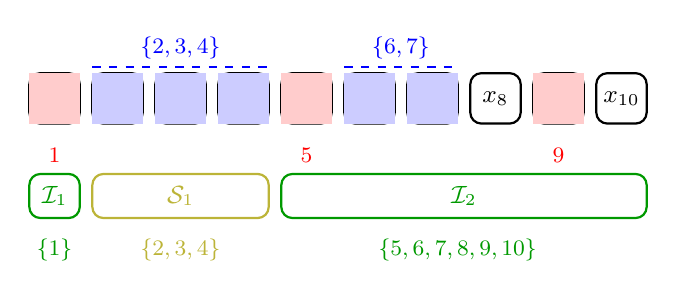
\begin{tikzpicture}[scale=0.8, every node/.style={align=center, font=\small}]
        % Draw the sequence of tokens
        \foreach \i in {1, 2, 3, 4, 5, 6, 7, 8, 9, 10} {
            \draw[rounded corners, thick] (\i, 0) rectangle (\i+0.8, 0.8) node[pos=.5] {$x_{\i}$};
        }

        % Highlight previously sampled tokens (M_<i)
        \foreach \i in {2, 3, 4, 6, 7} {
            \fill[blue!20] (\i, 0) rectangle (\i+0.8, 0.8);
        }

        % Highlight contiguous segments in M_<i
        \draw[thick, dashed, blue] (2, 0.9) -- (4.8, 0.9); % First segment: {2, 3, 4}
        \node[blue] at (3.4, 1.2) {\footnotesize $\{2, 3, 4\}$};

        \draw[thick, dashed, blue] (6, 0.9) -- (7.8, 0.9); % Second segment: {6, 7}
        \node[blue] at (6.9, 1.2) {\footnotesize $\{6, 7\}$};

        % Highlight current sampled tokens (M_i)
        \foreach \i in {1, 5, 9} {
            \fill[red!20] (\i, 0) rectangle (\i+0.8, 0.8);
        }

        % Label current tokens
        \node[red] at (1.4, -0.5) {\footnotesize $1$};
        \node[red] at (5.4, -0.5) {\footnotesize $5$};
        \node[red] at (9.4, -0.5) {\footnotesize $9$};

        % Draw intervals
        \draw[thick, green!60!black, rounded corners] (1, -1.5) rectangle (1.8, -0.8) node[pos=.5] {\small $\gI_1$};
        \node[green!60!black] at (1.4, -2) {\footnotesize $\{1\}$};

        \draw[thick, green!60!black, rounded corners] (5, -1.5) rectangle (10.8, -0.8) node[pos=.5] {\small $\gI_2$};
        \node[green!60!black] at (7.8, -2) {\footnotesize $\{5, 6, 7, 8, 9, 10\}$};

        \draw[thick, yellow!70!black, rounded corners] (2, -1.5) rectangle (4.8, -0.8) node[pos=.5] {\small $\gS_1$};
        \node[yellow!70!black] at (3.4, -2) {\footnotesize $\{2,3,4\}$};
    \end{tikzpicture}
    \caption{Illustration of the example for computing dependencies in the $n$-gram setting. Tokens $x_2, x_3, x_4, x_6, x_7$ (blue) represent the previously sampled location set $\gM_{<i}$, forming two contiguous segments: $\{2, 3, 4\}$ and $\{6, 7\}$. The current sampled locations $x_1, x_5, x_9$ (red) overlap with disjoint intervals $\gI_1 = \{1\}$ and $\gI_2 = \{5, 6, 7, 8, 9, 10\}$. The number of dependencies is computed as $\DEP_n(\gM_i, \gM_{<i}) = |\gM_i| - \text{(number of overlapping intervals)} = 3 - 2 = 1$.}
    \label{fig:dependencies}
\end{figure}


\noindent This example demonstrates how dependencies are computed, highlighting the interaction between previously sampled locations and the current reverse step. Such formalization is critical for understanding the efficiency and accuracy of discrete diffusion processes.

Finally, we extend this concept to define the total number of dependencies across an entire reverse process:

\begin{definition}[Number of Dependencies in a Reverse Process]
    Consider a reverse process $\tau = (\gM_1, \gM_2, \dots, \gM_N)$. Under the $n$-gram setting, the total number of dependencies in the process is defined as the sum of the dependencies across all steps:
    \[
    \DEP_n(\tau) = \sum_{i=1}^N \DEP_n(\gM_i, \gM_{<i}).
    \]
\end{definition}

Using the definition of $\DEP_n(\tau)$, we can bound the KL divergence between the distribution of sequences sampled under an instance of the reverse process and the ground-truth distribution in the $n$-gram setting.

\begin{lemma}[KL Divergence Upper Bound for the Instance of Reverse Process]
\label{lemma:kl_upper_ins_rev}
    Let $q$ denote the data distribution for sequences of length $L$, and let $p$ denote the distribution of sequences of length $L$ generated by reverse model $p_\theta$ via the reverse process $\tau$. Under \cref{ass:perfect_learning}, the following upper bound holds:
    \[
    \DKL{q}{p(\cdot|\tau)} \leq \DEP_n(\tau) \log |\gV|+L\eps_\mathrm{learning},
    \]
    where $\gV$ denote the vocabulary.
\end{lemma}

\begin{proof}
    Using \cref{lemma:kl_decomp_rev}, we have:
    $$\DKL{q}{p_\tau} = \sum_{i=1}^N \mathbb{E}_{\Tilde{\vx}_{<i}}\DKL{q(\Tilde{\vx}_i | \Tilde{\vx}_{<i})}{p_\tau(\Tilde{\vx}_i | \Tilde{\vx}_{<i})}.$$
    For each time step $t_i$:
    $$\mathbb{E}_{\Tilde{\vx}_{<i}}\DKL{q(\Tilde{\vx}_i | \Tilde{\vx}_{<i})}{p_\tau(\Tilde{\vx}_i | \Tilde{\vx}_{<i})}=\mathbb{E}_{\Tilde{\vx}_{<i}}\sum_{\Tilde{\vx}_i\in\gV^{|\gM_i|}}q(\Tilde{\vx}_i | \Tilde{\vx}_{<i})\log\frac{q(\Tilde{\vx}_i | \Tilde{\vx}_{<i})}{p_\tau(\Tilde{\vx}_i | \Tilde{\vx}_{<i})}.$$
    Given $\gM_i$ and $\gM_{<i}$, the tokens $\Tilde{\vx}_i$ at step $t_i$ can be partitioned into independently sampled token sets $\Tilde{\vx}_i^{(1)},\cdots,\Tilde{\vx}_i^{(m)}$ with $k_j$ denoting the size of each token set: 
    $$k_j=|\Tilde{\vx}_i^{(j)}|,\ j\in[m],\quad m=|\gM_i|-\DEP_n(\gM_i,\gM_{<i}).$$
    Using the independence, for each $\Tilde{\vx}_{<i}$, we can decompose the sum into:
    \begin{align*}
    \sum_{\Tilde{\vx}_i\in\gV^{|\gM_i|}}q(\Tilde{\vx}_i | \Tilde{\vx}_{<i})\log\frac{q(\Tilde{\vx}_i | \Tilde{\vx}_{<i})}{p_\tau(\Tilde{\vx}_i | \Tilde{\vx}_{<i})}&=\sum_{j=1}^m\sum_{\Tilde{\vx}_i^{(j)}\in\gV^{k_j}}q(\Tilde{\vx}_i^{(j)} | \Tilde{\vx}_{<i})\log\frac{q(\Tilde{\vx}_i^{(j)} | \Tilde{\vx}_{<i})}{p_\tau(\Tilde{\vx}_i^{(j)} | \Tilde{\vx}_{<i})}\\
    &=\sum_{j=1}^m\DKL{q(\Tilde{\vx}_i^{(j)} | \Tilde{\vx}_{<i})}{p_\tau(\Tilde{\vx}_i^{(j)} | \Tilde{\vx}_{<i}}.
    \end{align*}
    Under \cref{ass:perfect_learning}, the KL divergence between $q$ and $p_\theta$ is bounded by:
    $$\DKL{q_{0|t}(x_0^i \mid \vx_t)}{p_\mathbf{\theta}(x_0^i \mid \vx_t)} < \epsilon_\text{learning}, \quad \forall\ t \text{ and } \vx_t.$$
    By \cref{lemma:kl_mul_token_sample}, we know that:
    $$\DKL{q(\Tilde{\vx}_i^{(j)} | \Tilde{\vx}_{<i})}{p_\tau(\Tilde{\vx}_i^{(j)} | \Tilde{\vx}_{<i}}\leq (k_j-1)\log|\gV|+k_j\eps_\mathrm{learning}.$$
    Substituting back:
    $$\sum_{\Tilde{\vx}_i\in\gV^{|\gM_i|}}q(\Tilde{\vx}_i | \Tilde{\vx}_{<i})\log\frac{q(\Tilde{\vx}_i | \Tilde{\vx}_{<i})}{p_\tau(\Tilde{\vx}_i | \Tilde{\vx}_{<i})}\leq\sum_{j=1}^m(k_j-1)\log|\gV|+k_j\eps_\mathrm{learning}.$$
    Using the fact that
    $$\sum_{j=1}^m(k_j-1)=|\gM_i|-m=\DEP_n(\gM_i,\gM_{<i}),\quad \sum_{j=1}^mk_j=|\gM_i|$$
    we can obtain:
    $$\mathbb{E}_{\Tilde{\vx}_{<i}}\DKL{q(\Tilde{\vx}_i | \Tilde{\vx}_{<i})}{p_\tau(\Tilde{\vx}_i | \Tilde{\vx}_{<i})}\leq \DEP_n(\gM_i,\gM_{<i})\log|\gV|+|\gM_i|\eps_\mathrm{learning}.$$
    Thus, combined with the definition of $\DEP_n(\tau)$ and $p_\tau=p(\cdot|\tau)$, we can draw the final conclusion:
    \begin{align*}
        \DKL{q}{p(\cdot|\tau)} &\leq \sum_{i=1}^N\left(\DEP_n(\gM_i,\gM_{<i})\log|\gV|+|\gM_i|\eps_\mathrm{learning}\right)\\
        &=\DEP_n(\tau) \log |\gV|+L\eps_\mathrm{learning}.
    \end{align*}
    %In other words:
    %$$\DKL{q}{p(\cdot|\tau)} = \sum_{i=1}^N \DKL{q(\Tilde{\vx}_i | \Tilde{\vx}_{<i})}{p_\tau(\Tilde{\vx}_i | \Tilde{\vx}_{<i})}.$$
\end{proof}

The above Lemma directly leads to the bound for the KL divergence between the distribution of sequences generated by the reverse model with a given masking schedule and the ground-truth distribution in the $n$-gram setting.

\begin{lemma}[KL Divergence Upper Bound for a Masking Schedule]
\label{lemma:kl_bound_mask}
    Let $q$ denote the data distribution over sequences of length $L$, and let $p$ denote the distribution over sequences of length $L$ generated by the reverse model $p_\theta$ with masking schedule $\alpha_t$ and $N$ reverse steps. Under \cref{ass:perfect_learning}, the KL divergence between $q$ and $p$ satisfies the following upper bound:
    \[
    \DKL{q}{p} \leq \log |\gV| \sum_{i=1}^N \E_{\tau\sim\PROC(L, \alpha_t, N)} \DEP_n(\gM_i, \gM_{<i})+L\eps_\mathrm{learning}.
    \]
\end{lemma}

\begin{proof}
    By \cref{lemma:kl_upper_mask}, we can obtain:
    $$\DKL{q}{p} \leq \mathbb{E}_{\tau \sim \PROC(\alpha_t, N, L)} \DKL{q}{p(\cdot | \tau)}.$$
    Applying \cref{lemma:kl_upper_ins_rev} to the instances of reverse process, we can conclude that:
    \begin{align*}
    \DKL{q}{p} &\leq \mathbb{E}_{\tau \sim \PROC(\alpha_t, N,L)}\sum_{i=1}^N\DEP_n(\gM_i,\gM_{<i})\log|\gV|+L\eps_\mathrm{learning}\\
    &=\log |\gV| \sum_{i=1}^N \E_{\tau\sim\PROC(L, \alpha_t, N)} \DEP_n(\gM_i, \gM_{<i})+L\eps_\mathrm{learning}.
    \end{align*}
\end{proof}

For the final estimation, we need to derive an upper bound for the expected number of dependencies at each reverse step. First, we use Chernoff Bound to control the number of separators and new locations at each reverse step for a given masking schedule.

\begin{lemma}[Bounds on Separator and New Location Count at Each Reverse Step]
\label{lemma:bound_sep_new_rev}
    Given a sequence of length $L$, a masking schedule $\alpha_t$, and $N$ reverse steps. Assume that $L$ is divisible by $n-1$. Given the time step $t_i = \frac{N-i}{N}$, let $\NEW$ denote the number of locations sampled at step $t_i$, and $\SEP_n$ denote the number of separators in the previously sampled locations. Under the $n$-gram setting, the following bounds hold for $\NEW$ and $\SEP_n$:
    \begin{align*}
        \Pr\left(\SEP_n\leq \frac{Lp_i^{n-1}}{2(n-1)}\right)&\leq e^{-\frac{Lp_i^{n-1}}{8(n-1)}},\\
        \Pr\left(\NEW\geq 2L\delta_i\right)&\leq e^{-\frac{L\delta_i}{3}},
    \end{align*}
    where $p_i = \alpha_{t_{i-1}}$ and $\delta_i = \alpha_{t_i} - \alpha_{t_{i-1}}$.
\end{lemma}

\begin{proof}
Given a masking schedule $\alpha_t$, using the expression of true reverse process in \cref{eq:rev_proc} and $\alpha_1=0$, we can compute the probability $p^{(i)}$ of a token being sampled at time step $t_i$ to be:
$$p^{(i)}=\frac{\alpha_{t_i}-\alpha_{t_{i-1}}}{1-\alpha_{t_{i-1}}}\cdot\prod_{j=1}^{i-1}\frac{1-\alpha_{t_j}}{1-\alpha_{t_{j-1}}}=\alpha_{t_i} - \alpha_{t_{i-1}}=\delta_i.$$
Therefore, $\delta_i$ is the probability of a location being sampled at time step $t_i$. Summing up $\delta_i$, we can know that $p_i=\sum_{j=1}^{i-1}\delta_j$ is the probability of a location being sampled prior to time step $t_i$.

To derive a bound for $\SEP_n$, we partition the sequence into $\frac{L}{n-1}$ intervals, each of length $n-1$. For a given interval, the probability that all locations within the interval have been sampled prior to step $t_i$ is $p_i^{n-1}$. Define $X_j=1$ if the locations in the $j$-th interval have been sampled prior to $t_i$, and $X_j=0$ otherwise. The random variables $X_1,X_2,\cdots,X_{\frac{L}{n-1}}$ are independent and satisfy the following expectation:
$$\mathbb{E}_{\tau \sim \PROC(L, \alpha_t, N)}\sum_{j=1}^{\frac{L}{n-1}}X_j=\frac{Lp_i^{n-1}}{n-1}.$$
By the definition of $\SEP_n$, we know that:
$$\SEP_n\geq\sum_{j=1}^{\frac{L}{n-1}}X_j.$$
Applying \cref{lemma:chernoff} to the sum of $X_j$, we derive:
$$\Pr\left(\SEP_n\leq \frac{Lp_i^{n-1}}{2(n-1)}\right)\leq \Pr\left(\sum_{j=1}^{\frac{L}{n-1}}X_j\leq \frac{Lp_i^{n-1}}{2(n-1)}\right)\leq e^{-\frac{Lp_i^{n-1}}{8(n-1)}}.$$

Next, we consider the bound for $\NEW$. Given that the sequence contains $L$ locations and the probability of sampling any specific location at step $t_i$ is $\delta_i$, the expected number of new locations sampled at $t_i$ is given by:
$$\mathbb{E}_{\tau \sim \PROC(L, \alpha_t, N)}\NEW=L\delta_i.$$
Since the sampling of each location occurs independently, applying \cref{lemma:chernoff}, we have:
$$\Pr\left(\NEW\geq 2L\delta_i\right)\leq e^{-\frac{L\delta_i}{3}}.$$
\end{proof}

Using the above lemma, we can divide the estimation for the number of dependencies into three cases, and derive the bound case by case. This is achieved by using a variety of means and careful estimations.

\begin{lemma}[Upper Bound for the Expectation of Dependencies at Each Reverse Step]
\label{lemma:bound_dep_rev}
    Given a sequence of length $L$, a masking schedule $\alpha_t$, and $N$ reverse steps. Assume $L\delta_i>1$, then the expected number of dependencies at time step $t_i = \frac{N-i}{N}$ satisfies:
    \[
    \mathbb{E}_{\tau \sim \PROC(L, \alpha_t, N)} \DEP_n(\gM_i, \gM_{<i}) \leq \frac{9}{3+L\delta_i}+\frac{C(n-1)L\delta_i^2}{p_i^{n-1}},
    \]
    where $p_i = \alpha_{t_{i-1}}$, $\delta_i = \alpha_{t_i} - \alpha_{t_{i-1}}$, and $C$ is a constant.
\end{lemma}

\begin{proof}
By \cref{lemma:bound_sep_new_rev}, at step $t_i$, the following bounds hold:
\begin{align*}
        \Pr\left(\SEP_n\leq \frac{Lp_i^{n-1}}{2(n-1)}\right)&\leq e^{-\frac{Lp_i^{n-1}}{8(n-1)}},\\
        \Pr\left(\NEW\geq 2L\delta_i\right)&\leq e^{-\frac{L\delta_i}{3}}.
\end{align*}
Since $\DEP_n(\gM_i, \gM_{<i})\geq 0$, its expectation can be decomposed into three components:
\begin{align*}
    \mathbb{E}_{\tau \sim \PROC(L, \alpha_t, N)} \DEP_n(\gM_i, \gM_{<i})&=\Pr\left(\NEW\geq 2L\delta_i\right)\cdot \mathbb{E}_{\substack{\tau \sim \PROC(L, \alpha_t, N)\\ \NEW\geq 2L\delta_i}} \DEP_n(\gM_i, \gM_{<i})&\textbf{(Case 1)}\\
    &+\Pr\left(\SEP_n\leq \frac{Lp_i^{n-1}}{2(n-1)},\ \NEW< 2L\delta_i\right)\cdot \\
    &\qquad\mathbb{E}_{\substack{\tau \sim \PROC(L, \alpha_t, N)\\ \SEP_n\leq \frac{Lp_i^{n-1}}{2(n-1)}\\ \NEW< 2L\delta_i}} \DEP_n(\gM_i, \gM_{<i}) &\textbf{(Case 2)}\\
    &+\Pr\left(\SEP_n>\frac{Lp_i^{n-1}}{2(n-1)},\ \NEW< 2L\delta_i\right)\cdot \\
    &\qquad\mathbb{E}_{\substack{\tau \sim \PROC(L, \alpha_t, N)\\ \SEP_n>\frac{Lp_i^{n-1}}{2(n-1)}\\ \NEW<2L\delta_i}} \DEP_n(\gM_i, \gM_{<i})&\textbf{(Case 3)}
\end{align*}
We estimate these three cases separately.

\textbf{Case 1:} $\NEW\geq 2L\delta_i$.

By the definitions of $\DEP_n(\gM_i, \gM_{<i})$ and $\NEW$, we have:
$$\DEP_n(\gM_i, \gM_{<i})\leq |\gM_i|=\NEW.$$
Substituting this into the estimation, we obtain:
$$\Pr\left(\NEW\geq 2L\delta_i\right)\cdot \mathbb{E}_{\substack{\tau \sim \PROC(L, \alpha_t, N)\\ \NEW\geq 2L\delta_i}} \DEP_n(\gM_i, \gM_{<i})\leq \Pr\left(\NEW\geq 2L\delta_i\right)\cdot \mathbb{E}_{\substack{\tau \sim \PROC(L, \alpha_t, N)\\ \NEW\geq 2L\delta_i}} \NEW$$
Since $\DEP_n(\gM_i, \gM_{<i})\geq 0$, the expectation can be expressed as an integral of the tail probability:
$$\mathbb{E}_{\substack{\tau \sim \PROC(L, \alpha_t, N)\\ \NEW\geq 2L\delta_i}} \NEW=\int_{2L\delta_i}^{+\infty} \Pr\left(\NEW\geq x\mid\NEW\geq 2L\delta_i\right)\dd x.$$
It directly follows that:
\begin{align*}
    \Pr\left(\NEW\geq 2L\delta_i\right)\cdot \mathbb{E}_{\substack{\tau \sim \PROC(L, \alpha_t, N)\\ \NEW\geq 2L\delta_i}} \NEW &=\Pr\left(\NEW\geq 2L\delta_i\right)\cdot \int_{2L\delta_i}^{+\infty} \Pr\left(\NEW\geq x\mid\NEW\geq 2L\delta_i\right)\dd x\\
    &=\int_{2L\delta_i}^{+\infty} \Pr\left(\NEW\geq x\mid\NEW\geq 2L\delta_i\right)\Pr\left(\NEW\geq 2L\delta_i\right)\dd x\\
    &=\int_{2L\delta_i}^{+\infty}\Pr\left(\NEW\geq x\right)\dd x.
\end{align*}
Using the same trick as \cref{lemma:bound_sep_new_rev}, applying \cref{lemma:chernoff}, we can derive the bound for probability $\Pr\left(\NEW\geq x\right)$ as:
$$\Pr\left(\NEW\geq x\right)\leq e^{-\frac{(x-L\delta_i)^2}{x+L\delta_i}}.$$
Note that $\NEW\leq L$, we only need to consider $2\delta_i\leq 1$. In this case, we have:
\begin{align*}
    \int_{2L\delta_i}^{+\infty}\Pr\left(\NEW\geq x\right)\dd x \leq \int_{2L\delta_i}^{L}e^{-\frac{(x-L\delta_i)^2}{x+L\delta_i}}\dd x
\end{align*}
Let $y=x-L\delta_i\in[L\delta_i,L(1-\delta_i)]$, the integral can be rewritten as:
$$\int_{2L\delta_i}^{+\infty}\Pr\left(\NEW\geq x\right)\dd x \leq \int_{L\delta_i}^{L(1-\delta_i)}e^{-\frac{y^2}{y+2L\delta_i}}\dd y.$$
Observe that $y+2L\delta_i\leq 3y$, we can obtain:
$$\int_{2L\delta_i}^{+\infty}\Pr\left(\NEW\geq x\right)\dd x \leq \int_{L\delta_i}^{L(1-\delta_i)}e^{-\frac{y^2}{3y}}\dd y =3\left(e^{-\frac{L\delta_i}{3}}-e^{-\frac{L(1-\delta_i)}{3}}\right)=3e^{-\frac{L\delta_i}{3}}\left(1-e^{-\frac{L(1-2\delta_i)}{3}}\right).$$
Using the fact that $e^{-x}\leq\frac{1}{1+x}$ for $x\geq 0$, we have the upper bound:
$$3e^{-\frac{L\delta_i}{3}}\left(1-e^{-\frac{L(1-2\delta_i)}{3}}\right)\leq 3e^{-\frac{L\delta_i}{3}}\leq \frac{9}{3+L\delta_i}.$$
Combining the above results, we know that:
$$\Pr\left(\NEW\geq 2L\delta_i\right)\cdot \mathbb{E}_{\substack{\tau \sim \PROC(L, \alpha_t, N)\\ \NEW\geq 2L\delta_i}} \DEP_n(\gM_i, \gM_{<i})\leq \frac{9}{3+L\delta_i}.$$

\textbf{Case 2:} $\SEP_n\leq \frac{Lp_i^{n-1}}{2(n-1)}$ and $ \NEW<2L\delta_i$.

Similar to Case 1, we have:
$$\DEP_n(\gM_i, \gM_{<i})\leq\NEW<2L\delta_i,$$
so the expectation also follows:
$$\mathbb{E}_{\substack{\tau \sim \PROC(L, \alpha_t, N)\\ \SEP_n\leq \frac{Lp_i^{n-1}}{2(n-1)}\\ \NEW< 2L\delta_i}} \DEP_n(\gM_i, \gM_{<i})< 2L\delta_i.$$
Using the probability bound, it follows that:
$$\Pr\left(\SEP_n\leq \frac{Lp_i^{n-1}}{2(n-1)},\ \NEW< 2L\delta_i\right)\leq\Pr\left(\SEP_n\leq \frac{Lp_i^{n-1}}{2(n-1)}\right)\leq e^{-\frac{Lp_i^{n-1}}{8(n-1)}}.$$
Since $e^{-x}\leq\frac{1}{1+x}$ for $x\geq 0$:
$$e^{-\frac{Lp_i^{n-1}}{8(n-1)}}\leq\frac{8(n-1)}{Lp_i^{n-1}+8(n-1)}.$$
Combining these results, we obtain:
$$\Pr\left(\SEP_n\leq \frac{Lp_i^{n-1}}{2(n-1)},\ \NEW< 2L\delta_i\right)\cdot\mathbb{E}_{\substack{\tau \sim \PROC(L, \alpha_t, N)\\ \SEP_n\leq \frac{Lp_i^{n-1}}{2(n-1)}\\ \NEW< 2L\delta_i}} \DEP_n(\gM_i, \gM_{<i})\leq \frac{16(n-1)L\delta_i}{Lp_i^{n-1}+8(n-1)}.$$

\textbf{Case 3:} $\SEP_n>\frac{Lp_i^{n-1}}{2(n-1)}$ and $ \NEW<2L\delta_i$.

Apparently, we have:
$$\Pr\left(\SEP_n>\frac{Lp_i^{n-1}}{2(n-1)},\ \NEW< 2L\delta_i\right)\leq 1.$$
Given $a,b$, let $\mathbb{E}_{a,b}\DEP_n(\gM_i, \gM_{<i})$ denote the expectation of $\DEP_n(\gM_i, \gM_{<i})$ under the condition of $\SEP_n=a$ and $ \NEW=b$. In other words:
$$\mathbb{E}_{a,b}\DEP_n(\gM_i, \gM_{<i})=\mathbb{E}_{\substack{\tau \sim \PROC(L, \alpha_t, N)\\ \SEP_n=a\\ \NEW=b}} \DEP_n(\gM_i, \gM_{<i}).$$
Since all the locations are sampled independently, and $\DEP_n(\gM_i, \gM_{<i})$ depends only on the relative positions of separators in $\gM_{<i}$ and the new locations in $\gM_i$, the expectation $\mathbb{E}_{a,b}\DEP_n(\gM_i, \gM_{<i})$ only depends on the ordering of separators and new locations.

Assume $x_1,\cdots,x_{a+b}$ are $a+b$ positions (not locations) in order. We can regard the process of ordering separators and new locations as the process of choosing $b$ positions randomly from $x_j$. For $1\leq j\leq a+b-1$, define $X_j=1$ if $x_j$ and $x_{j+1}$ are both new locations, and $X_j=0$ otherwise. By the definition of $\DEP_n(\gM_i, \gM_{<i})$, we can obtain:
$$\DEP_n(\gM_i, \gM_{<i})=\sum_{j=1}^{a+b-1}X_j.$$
Since the $b$ new locations are chosen randomly, the probability of $X_j=1$ can be calculated as:
$$\Pr(X_j=1)=\frac{C_{a+b-2}^{b-2}}{C_{a+b}^{b}}=\frac{b(b-1)}{(a+b)(a+b-1)}.$$
Therefore, the expectation of $X_j$ is:
$$\mathbb{E}X_j=\frac{b(b-1)}{(a+b)(a+b-1)}.$$
Summing up, we have:
$$\mathbb{E}_{a,b}\DEP_n(\gM_i, \gM_{<i})=\mathbb{E}\sum_{j=1}^{a+b-1}X_j=(a+b-1)\mathbb{E}X_1=\frac{b(b-1)}{a+b}.$$
Since $a>\frac{Lp_i^{n-1}}{2(n-1)}$ and $b<2L\delta_i$, we can derive the upper bound for any $a,b$:
$$\frac{b(b-1)}{a+b}\leq \frac{b(b-1)}{\frac{Lp_i^{n-1}}{2(n-1)}+b} \leq\frac{2L\delta_i(2L\delta_i-1)}{\frac{Lp_i^{n-1}}{2(n-1)}+2L\delta_i}\leq \frac{8(n-1)L\delta_i^2}{p_i^{n-1}+4(n-1)\delta_i}.$$
Since this holds for all $a$ and $b$, we can obtain:
\begin{align*}
    &\quad\Pr\left(\SEP_n>\frac{Lp_i^{n-1}}{2(n-1)},\ \NEW< 2L\delta_i\right)\cdot\mathbb{E}_{\substack{\tau \sim \PROC(L, \alpha_t, N)\\ \SEP_n>\frac{Lp_i^{n-1}}{2(n-1)}\\ \NEW<2L\delta_i}} \DEP_n(\gM_i, \gM_{<i})\\
    &\leq \mathbb{E}_{\substack{\tau \sim \PROC(L, \alpha_t, N)\\ \SEP_n>\frac{Lp_i^{n-1}}{2(n-1)}\\ \NEW<2L\delta_i}} \DEP_n(\gM_i, \gM_{<i})\\
    &=\sum_{a>\frac{Lp_i^{n-1}}{2(n-1)},\ b<2L\delta_i}\Pr(\SEP_n=a, \NEW=b)\cdot\mathbb{E}_{a,b}\DEP_n(\gM_i, \gM_{<i})\\
    &\leq \frac{8(n-1)L\delta_i^2}{p_i^{n-1}+4(n-1)\delta_i}.
\end{align*}

\textbf{Summarize the above proof:}

Combining the above three cases, we can obtain:
$$\mathbb{E}_{\tau \sim \PROC(L, \alpha_t, N)} \DEP_n(\gM_i, \gM_{<i}) \leq \frac{9}{3+L\delta_i}+\frac{16(n-1)L\delta_i}{Lp_i^{n-1}+8(n-1)}+\frac{8(n-1)L\delta_i^2}{p_i^{n-1}+4(n-1)\delta_i}.$$
If we have the assumption $L\delta_i\geq 1$, it is easy to find that:
\begin{align*}
    \mathbb{E}_{\tau \sim \PROC(L, \alpha_t, N)} \DEP_n(\gM_i, \gM_{<i}) &\leq \frac{9}{3+L\delta_i}+\frac{16(n-1)\delta_i}{p_i^{n-1}}+\frac{8(n-1)L\delta_i^2}{p_i^{n-1}}\\
    &\leq \frac{9}{3+L\delta_i}+\frac{16(n-1)L\delta_i^2}{p_i^{n-1}}+\frac{8(n-1)L\delta_i^2}{p_i^{n-1}}\\
    &\leq \frac{9}{3+L\delta_i}+\frac{C(n-1)L\delta_i^2}{p_i^{n-1}}.
\end{align*}
Where $C=24$ is a constant.

\end{proof}

Finally, we can derive the upper bound for the KL divergence between the distribution of sequences generated by the
reverse model and the ground-truth distribution in the n-gram setting.

\begin{lemma}[Efficient Sampling with Small KL Divergence]
\label{lemma:effi_kl_bound}
    Let $q$ denote the data distribution over sequences of length $L$, and let $p$ denote the distribution over sequences of length $L$ generated by the reverse model $p_\theta$ with a masking schedule $\alpha_t$ and $N$ reverse steps. Assume that $p_\theta$ satisfies \cref{ass:perfect_learning}. For any $\epsilon > 0$, there exists a masking schedule $\alpha_t$ such that, for $L\geq \frac{3C(n-1)}{\eps^{n+\frac{1}{2}}}$, with $N = O\left(\frac{n-1}{\eps^{n}}\right)$ sampling steps, the KL divergence between $q$ and $p$ satisfies:
    $$\frac{\DKL{q}{p}}{L\log|\gV|} \leq 4\eps +\frac{\eps_\mathrm{learning}}{\log|\gV|}.$$
\end{lemma}

\begin{proof}
    By \cref{lemma:kl_bound_mask}, we know that:
    $$\DKL{q}{p} \leq \log |\gV| \sum_{i=1}^N \E_{\tau\sim\PROC(L, \alpha_t, N)} \DEP_n(\gM_i, \gM_{<i})+L\eps_\mathrm{learning}.$$
    Note that at step $t_1$, the reverse process can be bounded using \cref{lemma:kl_mul_token_sample}. By reviewing our proof process, it is easy to see that we can substitute $\DEP_n(\gM_1, \gM_{<1})$ for $(|\gM_1|-1)\log |\gV|$, where $\gV$ stands for the vocabulary. By the definition of $\delta_i$, we know that:
    $$\E_{\tau\sim\PROC(L, \alpha_t, N)} (|\gM_1|-1)\log |\gV|=(\delta_1L-1)\log |\gV|.$$
    Applying \cref{lemma:bound_dep_rev} to $\DEP_n(\gM_i, \gM_{<i})$, if $L\delta_i\geq 1$, we can obtain:
    $$\DKL{q}{p}\leq \delta_1\log |\gV|+\log |\gV| \sum_{i=2}^N\left(\frac{9}{3+L\delta_i}+\frac{C(n-1)L\delta_i^2}{p_i^{n-1}}\right)+L\eps_\mathrm{learning}.$$
    By the definition of $p_i$, we know that $p_2=\delta_1$. For any small $\eps>0$, consider the following masking schedule:
    %$$\delta_1=\frac{\eps}{\log |\gV|},\quad \delta_i=\delta=\frac{\eps^n}{C(n-1)(\log|\gV|)^n},\quad p_i=\delta_1+(i-2)\delta,\quad\forall i\geq 2.$$
    $$\delta_1=\eps,\quad \delta_i=\delta=\frac{\eps^n}{C(n-1)},\quad p_i=\delta_1+(i-2)\delta,\quad\forall i\geq 2.$$
    Then, for $L\geq \frac{1}{\delta}$, the KL divergence can be bounded by:
    \begin{align*}
        \frac{\DKL{q}{p}}{L\log|\gV|}&\leq \eps+\frac{9(N-1)}{L(3+L\delta)}+\sum_{i=2}^N \frac{C(n-1)\delta^2}{p_i^{n-1}}+\frac{\eps_\mathrm{learning}}{\log|\gV|}\\
        &=\eps+\frac{9(1-\delta_1)}{L\delta(3+L\delta)}+\frac{C(n-1)\delta^2}{\delta_1^{n-1}}+\sum_{i=1}^{N-2} \frac{C(n-1)\delta^2}{(\delta_1+i\delta)^{n-1}}+\frac{\eps_\mathrm{learning}}{\log|\gV|}.\\
        &\leq \eps+\frac{9}{L\delta(3+L\delta)}+\frac{C(n-1)\delta^2}{\delta_1^{n-1}}+\sum_{i=1}^{N-2} \frac{C(n-1)\delta^2}{(\delta_1+i\delta)^{n}}+\frac{\eps_\mathrm{learning}}{\log|\gV|}.
    \end{align*}
    By simple calculations, we know that:
    $$\frac{9}{L\delta(3+L\delta)}\leq \eps,\quad \text{if }L\geq \frac{3}{\delta\eps^{\frac{1}{2}}}.$$
    It is clear that $\delta\leq 1$, so:
    $$\frac{C(n-1)\delta^2}{\delta_1^{n-1}}\leq \eps\delta\leq\eps.$$
    Since $x^{-n}$ is convex on $[0,+\infty)$, the accumulation can be bounded by:
    \begin{align*}
        \sum_{i=1}^{N-2} \frac{C(n-1)\delta^2}{(\delta_1+i\delta)^n}&=C(n-1)\delta^{2-n}\sum_{i=1}^{N-2}\frac{1}{(\frac{\delta_1}{\delta}+i)^n}\\
        &\leq C(n-1)\delta^{2-n}\sum_{i=1}^{N-2}\int_{x=0}^{+\infty}\frac{1}{(\frac{\delta_1}{\delta}+x)^n\dd x}\\
        &=C(n-1)\delta^{2-n}\cdot\frac{1}{n-1}\left(\frac{\delta}{\delta_1}\right)^{n-1}\\
        &=\frac{C\delta}{\delta_1^{n-1}}\\
        &\leq\eps.
    \end{align*}
    Combining the above, we have:
    $$\frac{\DKL{q}{p}}{L\log|\gV|}\leq 4\eps+\frac{\eps_\mathrm{learning}}{\log|\gV|}.$$
    Meanwhile, the time step is limited by:
    $$N=1+\frac{1-\delta_1}{\delta}=O\left(\frac{n-1}{\eps^n}\right),$$
    and the lower bound for $L$:
    $$L\geq \frac{3}{\delta\eps^{\frac{1}{2}}}=\frac{3C(n-1)}{\eps^{n+\frac{1}{2}}}.$$

\end{proof}

Combining the above lemmas, we can prove \cref{thm:acceleration_ngram} by breaking the expression of $\log\PPL(p)$ into two parts.

\begin{theorem}[$\PPL$ Bounds for $n$-Gram Language Generation]
    For any $n$-gram language $q$ and any $\epsilon > 0$, let $p_\mathsf{\theta}$ denote the reverse model and $L$ denote the sequence length. The distribution over sequences generated by $p_\mathsf{\theta}$ is denoted as $p$. For any $L>O\big( \frac{n-1}{\epsilon^{n+0.5}}\big)$, under \cref{ass:perfect_learning}, there exists a masking schedule $\alpha_t$ such that, with $N = O\big( \frac{n-1}{\epsilon^n}\big)$ sampling steps, the perplexity of the MDM is upper-bounded by:
    $$\log\PPL(p) \leq \log\PPL(q) + \epsilon_\text{learning} + 4\epsilon\log |\gV|.$$
\end{theorem}

\begin{proof}
    By \cref{lemma:effi_kl_bound}, for any $L>O\big( \frac{n-1}{\epsilon^{n+0.5}}\big)$, there exists a masking schedule $\alpha_t$ with $N = O\big( \frac{n-1}{\epsilon^n}\big)$ sampling steps satisfying:
    $$\frac{\DKL{q}{p}}{L\log|\gV|} \leq 4\eps+\frac{\eps_\mathrm{learning}}{\log|\gV|}.$$
    In other words:
    $$\frac{1}{L}\mathbb{E}_{\vx \sim q}
    \log \frac{q(\vx)}{p(\vx)}\leq 4\eps\log|\gV|+\eps_\mathrm{learning}.$$
    By the definition of $\PPL$, we have:
    $$\log\PPL(p) = \mathbb{E}_{\vx \sim q} -\frac{\log p(\vx)}{|\vx|}=\frac{1}{L}\mathbb{E}_{\vx \sim q}\left(-\log q(\vx)+\log\frac{q(\vx)}{p(\vx)}\right).$$
    Note that:
    $$\log\PPL(q) = \mathbb{E}_{\vx \sim q} -\frac{\log q(\vx)}{|\vx|}=\frac{1}{L}\mathbb{E}_{\vx \sim q}-\log q(\vx).$$
    We can obtain:
    $$\log\PPL(p) \leq \log\PPL(q) + \epsilon_\text{learning} + 4\epsilon\log |\gV|.$$
\end{proof}


\section{Proof for \cref{thm:pos_hmm} and \cref{thm:negative}}
\subsection{Proof for \cref{thm:pos_hmm}}
\label{app:proof_hmm_pos}
In this section, we aim to derive the upper bound for the $\SER$ of generated sequences with sufficient reverse steps. First, we argue that, given a making schedule $\alpha_t$, with sufficient steps, the probability of sampling multiple locations in the sequence at the same time can be very low.

\begin{lemma}[Low Probability of Simultaneous Sampling with Sufficient Steps]
\label{lemma:prob_mul_suff}
    Given a sequence of length $L$ and a masking schedule $\alpha_t$. For any $\eps>0$, there exists $N_0$, such that for any $N\geq N_0$, with $N$ reverse steps, the probability $p_\mathrm{mul}$ of sampling multiple locations in the sequence at the same time satisfies:
    $$p_\mathrm{mul}<\eps.$$
\end{lemma}

\begin{proof}
    By \cref{lemma:bound_sep_new_rev}, we know that the probability of a location being sampled at time step $t_i=\frac{N-i}{N}$ is:
    $$\delta_i=\alpha_{t_i}-\alpha_{t_{i-1}}=\alpha_\frac{N-i}{N}-\alpha_\frac{N-i+1}{N}.$$
    Since all the locations are sampled independently, for two distinct locations $i\neq j$ in the sequence, the probability that $i$ and $j$ are sampled simultaneously is:
    $$p_{i,j}=\sum_{i=1}^{N}\delta_i^2.$$
    Summing up $p_{i,j}$, the probability of having two locations a=sampled simultaneously can be bounded by:
    $$p_\mathrm{mul}\leq \frac{L(L-1)}{2}\cdot\sum_{i=1}^{N}\delta_i^2$$
    Since $\alpha_t$ is continuous on $[0,1]$, we know that it is uniformly continuous. Therefore, for any $\eps>0$, there exists $N_0>0$ that satisfies:
    $$|\alpha_x-\alpha_y|<\frac{2\eps}{L(L-1)}, \quad\forall x,y\in [0,1], |x-y|<\frac{1}{N_0}.$$
    In this case, for $N>N_0$, we know that:
    $$|\delta_i|=|\alpha_\frac{N-i}{N}-\alpha_\frac{N-i+1}{N}|<\frac{2\eps}{L(L-1)},\quad\forall i\in [N].$$
    Combining with the fact that $\sum_{i=1}^N\delta_i=1$, we can obtain:
    $$p_\mathrm{mul}\leq \frac{L(L-1)}{2}\cdot\sum_{i=1}^{N}\delta_i\cdot\max_{j\in [N]}\delta_j<\eps.$$
\end{proof}

Next, we consider the $\SER$ increase due to the learning error. Specifically, we only investigate the case where all the locations are sampled at different steps.

\begin{lemma}[Accurate Step-by-Step Generation with Low Learning Error]
\label{lemma:acc_gen}
    Let $q$ denote any HMM, and let $p_\mathsf{\theta}$ represent the reverse model under an arbitrary masking schedule, where $L$ is the sequence length. Let $p$ denote the distribution over sequences generated by $p_\mathsf{\theta}$. Under \cref{ass:perfect_learning} with a learning error $\epsilon_\text{learning} < \frac{\delta}{L},\ \delta>0$, and given an instance of reverse process $\tau=(\gM_1,\gM_2,\cdots,\gM_N)$ with $|\gM_i|\leq 1$, let $p_\mathrm{acc}$ denote the probability of generating a valid sequence. Then $p_\mathrm{acc}$ satisfies:
    $$p_\mathrm{acc}\geq e^{-\delta}.$$
\end{lemma}

\begin{proof}
    Since $|\gM_i|\leq 1$, we only need to consider the steps where one token is sampled. Let $\Tilde{\vx}_t$ denote the previously sampled tokens, and $\Tilde{x}_t$ denote the token sampled at the current step. If $\Tilde{\vx}_t$ is can later form a valid sequence, let $\gX_t$ denote the set of valid choices for $\Tilde{x}_t$. In other words, if $\Tilde{x}_t\in \gX_t$, then the combination of $\Tilde{\vx}_t$ and $\Tilde{x}_t$ is can later form a valid sequence, or more intuitively:
    $$q_{0|t}(\Tilde{x}_t\mid\Tilde{\vx}_t)>0.$$
    Under \cref{ass:perfect_learning}, we know that:
    $$\DKL{q_{0|t}(x_t \mid \Tilde{\vx}_t)}{p_\mathbf{\theta}(x_t \mid \Tilde{\vx}_t)} < \epsilon_\text{learning}.$$
    Since it is assumed that $0\log 0=0$, we have:
    $$\sum_{x_t\in\gX_t}q_{0|t}(x_t \mid \Tilde{\vx}_t)\log\frac{q_{0|t}(x_t \mid \Tilde{\vx}_t)}{p_\theta(x_t \mid \Tilde{\vx}_t)}<\eps_\text{learning}.$$
    Equivalently, we have:
    $$-\eps_\text{learning}<\sum_{x_t\in\gX_t}q_{0|t}(x_t \mid \Tilde{\vx}_t)\log\frac{p_\theta(x_t \mid \Tilde{\vx}_t)}{q_{0|t}(x_t \mid \Tilde{\vx}_t)}.$$
    Due to the concavity of $\log x$, by Jensen's Inequality, we can obtain:
    $$\sum_{x_t\in\gX_t}q_{0|t}(x_t \mid \Tilde{\vx}_t)\log\frac{p_\theta(x_t \mid \Tilde{\vx}_t)}{q_{0|t}(x_t \mid \Tilde{\vx}_t)}\leq \log\left(\sum_{x_t\in\gX_t}q_{0|t}(x_t \mid \Tilde{\vx}_t)\cdot \frac{p_\theta(x_t \mid \Tilde{\vx}_t)}{q_{0|t}(x_t \mid \Tilde{\vx}_t)}\right) =\log\sum_{x_t\in\gX_t}p_\theta(x_t \mid \Tilde{\vx}_t).$$
    Therefore, the probability that each step remains valid satisfies:
    $$\sum_{x_t\in\gX_t}p_\theta(x_t \mid \Tilde{\vx}_t)\geq e^{-\eps_\text{learning}}\geq e^{-\frac{\delta}{L}}.$$
    Since there are $L$ locations in the sequence, the probability of generating a valid sequence is bounded by:
    $$p_\mathrm{acc}\geq (e^{-\frac{\delta}{L}})^L=e^{-\delta}.$$
\end{proof}

Combining the above lemmas, we can derive the upper bound of $\SER$ by taking sufficient reverse steps and small learning error.

\begin{theorem}[Accurate Generation of HMM with Sufficient Steps]
    Let $q$ denote any HMM, and let $p_\mathsf{\theta}$ represent the reverse model under an arbitrary masking schedule, where $L$ is the sequence length. Let $p$ denote the distribution over sequences generated by $p_\mathsf{\theta}$. Under \cref{ass:perfect_learning} with a learning error $\epsilon_\text{learning} < O(\frac{\delta}{L})$, and given a sufficient number of reverse steps, the sequence error rate $\operatorname{SER}(p)$ of the generated text satisfies 
    \[
    \operatorname{SER}(p) \leq  \delta.
    \]
\end{theorem}

\begin{proof}
    For $\delta>0$, we know that:
    $$1-\delta<c.$$
    By \cref{lemma:prob_mul_suff}, given the masking schedule $\alpha_t$, there exists $N_0$, for $N>N_0$ and $N$ reverse steps, the probability of sampling multiple locations in the sequence at the same time is bounded by:
    $$p_\mathrm{mul}<1-\frac{1-\delta}{e^{-\delta}}.$$
    In other words, the probability of sampling all the locations at different steps is at least $\frac{1-\delta}{e^{-\delta}}$. By \cref{lemma:acc_gen}, for each reverse process which satisfies that all the locations are sampled at different steps, the probability of generating a valid sequence is lower bounded by:
    $$p_\mathrm{acc}\geq e^{-\delta}.$$
    Therefore, the sequence error rate $\SER$ satisfies:
    $$\SER(p)\leq 1-\frac{1-\delta}{e^{-\delta}}\cdot e^{-\delta}= \delta.$$
\end{proof}

\subsection{Proof for \cref{thm:negative}}
\label{app:proof_neg}
In the section, we aim to find an example (\cref{exa:interval}) with high sequence error rate. To present this example, we begin with a special class of languages defined under the interval setting:

\begin{definition}[Interval Setting]
\label{def:interval_setting}
Consider a sequence of length $L$, which is divided equally into $M$ intervals $\gI_1,\gI_2,\cdots,\gI_M$, each of length $l=\frac{L}{M}\geq 2$. Given a masking schedule $\alpha_t$, an instance of reverse process $\tau=(\gM_1,\gM_2,\cdots,\gM_N)$ is defined by \cref{def:ins_rev}. For any two locations within different intervals, their corresponding tokens are independent from each other. In other words, let $\Tilde{\vx}_i^{(j)}$ denote the new tokens in $\gM_i\cap\gI_j$, $\Tilde{\vx}_{<i}^{(j)}$ denote the previously sampled tokens in $\gM_{<i}\cap\gI_j$, and $p$ denote the distribution over sequences generated by the reverse model with reverse process $\tau$, then for time step $t_i=\frac{N-i}{N}$:
$$p(\Tilde{\vx}_i^{(j)}|\Tilde{\vx}_{<i})=p(\Tilde{\vx}_i^{(j)}|\Tilde{\vx}_{<i}^{(j)}).$$
In this case, we have:
$$p(\vx)=\prod_{j=1}^{M}p(\vx^{(j)})=\prod_{j=1}^{M}\prod_{i=1}^{N}p(\Tilde{\vx}_i^{(j)}|\Tilde{\vx}_{<i}^{(j)}).$$
We denote the above setting as $\operatorname{Inter}(L,l,\alpha_t)$.
\end{definition}

% \begin{definition}[Interval Setting]
% \label{def:interval_setting}
% Consider a sequence of length $L$, which is divided equally into $N$ intervals, each of length $l=L/N$. At each step, one or two previously unselected positions, denoted $i$ or $(i,j)$ with $ i\neq j$, are randomly chosen from the sequence. Random variables are then sampled according to
% $$X_i \sim q_i(X_{I_i}), \quad \text{and independently, } X_j \sim q_j(X_{I_j}),$$
% where $X_{I_i}$ represents the set of previously sampled random variables within the interval of $i$, and similarly for $X_{I_j}$.

% Let $M$ be the total number of steps in which two positions are sampled simultaneously. The overall setting is denoted as $\operatorname{Inter}(L,N,M)$.
% \end{definition}

Under the interval setting defined above, we can control the probability of sampling simultaneously in the same interval.

\begin{lemma}[Simultaneous Sampling Probability for an Interval]
\label{lemma:simul_prob_inter}
    Consider the interval setting $\operatorname{Inter}(L,l,\alpha_t)$. For each interval $\gI_j$ of length $l$, let $h_j$ denote the probability that all the locations in $\gI_j$ are sampled in different time steps. Then, 
    % for $\alpha_t$ satisfying $\max\delta_i\leq \frac{2}{l}$, 
    $h_j$ can be bounded by:
    % $$h_j\leq \left(1-\frac{1}{N}\right)^{l-1},$$
    % and for all $\alpha_t$:
    $$h_j\leq 1-\frac{1}{N}.$$
\end{lemma}

\begin{proof}
    Let $\delta_i=\alpha_{t_i}-\alpha_{t_{i-1}}$. Similar to \cref{lemma:bound_sep_new_rev}, we know that $\delta_i$ is the probability of a location being sampled at time step $t_i$. Take the first location in $|\gI_j|$, denote it as $X_1$, and let $X_2,\cdots,X_l$ denote the rest $l-1$ locations in $\gI_j$. If $X_1$ is sampled at step $t_i$, then $X_2,\cdots,X_l$ must be sampled at time steps other than $t_i$. Therefore, $h_j$ can be bounded by:
    $$h_j\leq \sum_{i=1}^{N}\delta_i(1-\delta_i)^{l-1}\leq\sum_{i=1}^{N}\delta_i(1-\delta_i).$$
    Let $f(\delta)=\delta(1-\delta)$. Note that we have:
    $$f''(\delta)=-2\leq 0,$$
    which indicates that $f(\delta)$ is concave. Using Jensen's Inequality, we can obtain:
    $$h_j\leq \sum_{i=1}^{N}f(\delta_i)\leq Nf\left(\frac{1}{N}\right)=1-\frac{1}{N}.$$
    
    % $$h_j\leq \sum_{i=1}^{N}\delta_i(1-\delta_i)^{l-1}.$$
    % Let $f(\delta)=\delta(1-\delta)^{l-1}$. Note that for $l\delta\leq 2$, we have:
    % $$f''(\delta)=-(l-1)(2-l\delta)(1-\delta)^{l-3}\leq 0,$$
    % which indicates that $f(\delta)$ is concave. Using Jensen's Inequality, we can obtain:
    % $$h_j\leq \sum_{i=1}^{N}f(\delta_i)\leq Nf\left(\frac{1}{N}\right)=\left(1-\frac{1}{N}\right)^{l-1}.$$
    
    % In the other hand, for any $\alpha_t$, note that:
    % $$h_j\leq \sum_{i=1}^{N}\delta_i(1-\delta_i)^{l-1}\leq \sum_{i=1}^{N}\delta_i(1-\delta_i).$$
    % Using similar tricks as before, we can get:
    % $$h_j\leq 1-\frac{1}{N}.$$

\end{proof}

Using the above lemma, if we assume that sampling simultaneously in one interval increases $\SER$, then we can derive an lower bound for $\SER(p)$.

\begin{lemma}[$\SER$ bound for Interval Setting]
\label{lemma:acc_inter}
    Consider the interval setting $\operatorname{Inter}(L,l,\alpha_t)$. Assume that sampling simultaneously in the same interval introduces an error with probability at least $p_0$, and other actions do not reduce error. In other words, if two locations in an interval are both sampled at step $t_i$, then there is a probability of $p_e$ that the sequence will not be accurate afterwards. In this case, let $p$ denote the distribution over sequences of length $L$ generated by the reverse model with masking schedule $\alpha_t$ and $N$ reverse steps. We have the following bound for $\SER$: 
    % if $\max\delta_i\leq \frac{2}{l}, N\geq (l-1)(l-2)$ and $l\geq 2$, we have:
    % $$\operatorname{ACC}(p)\leq \left(1-\frac{(l-2)p_e}{N}\right)^{L/l}.$$
    % In other cases:
    $$\SER(p)\geq 1-\left(1-\frac{p_e}{N}\right)^{L/l}.$$
\end{lemma}

\begin{proof}
    By \cref{lemma:simul_prob_inter}, we can obtain that for each interval $\gI_j$, the probability $p_\textrm{error}^{(j)}$ of generating an error in $\gI_j$ is lower-bounded by:
    $$p_\textrm{error}^{(j)}\geq p_e(1-h_j)\geq\frac{p_e}{N}.$$
    % $$\begin{cases}
    %     p_\textrm{error}^{(j)}\geq p_e\left(1-(1-\frac{1}{N})^{l-1}\right), &\max\delta_i\leq \frac{2}{l},\\
    %     p_\textrm{error}^{(j)}\geq \frac{p_e}{N}, &\textit{otherwise}.
    % \end{cases}$$
    % Expanding the formula, we have:
    % \begin{align*}
    %     1-(1-\frac{1}{N})^{l-1}&=\left(1-(1-\frac{1}{N})\right)\cdot \left(1+(1-\frac{1}{N})+\cdots+(1-\frac{1}{N})^{l-2}\right)\\
    %     &\geq \frac{l-1}{N}\left(1-\frac{1}{N}\right)^{l-2}\\
    %     &\geq \frac{l-1}{N}\left(1-\frac{l-2}{N}\right).
    % \end{align*}
    % If $N\geq (l-1)(l-2)$, we know that:
    % $$1-(1-\frac{1}{N})^{l-1}\geq \frac{l-2}{N}$$
    Due to the independence between different intervals, the accuracy $\SER(p)$ can be calculated as:
    $$\SER(p)=1-\prod_{j=1}^{M}(1-p_\textrm{error}^{(j)}).$$
    Therefore, we have the bound:
    $$\SER(p)\geq 1-\left(1-\frac{p_e}{N}\right)^{L/l}.$$
    % Therefore, for $\max\delta_i\leq \frac{2}{l}, N\geq (l-1)(l-2)$ and $l\geq 2$, we know that:
    % $$\operatorname{ACC}(p)\leq \left(1-\frac{(l-2)p_e}{N}\right)^{L/l}.$$
    % And in other cases, we have:
    % $$\operatorname{ACC}(p)\leq \left(1-\frac{p_e}{N}\right)^{L/l}.$$
\end{proof}

% \begin{lemma}[Interval Sampling Probability Bound]
% \label{lemma:interval_bound}
% Consider the setting $\operatorname{Inter}(L,N,M)$. Assume that there are $k$ unsampled positions remaining, and two positions are sampled simultaneously. Let $p(k)$ denote the probability that both sampled positions belong to the same interval. Then $p(k)$ satisfies
% $$p(k)\geq \max\left\{0,\frac{k-N}{(k-1)N}\right\}.$$
% \end{lemma}

% \begin{proof}
% The probability \( p(k) \) of selecting two positions within the same interval is given by:
% \[
% p(k) = \frac{1}{k(k-1)} \sum_{i=1}^N u_i(u_i-1),
% \]
% where \( u_i \) is the number of unsampled positions in the \( i \)-th interval, and \( \sum_{i=1}^N u_i = k \).
% By the AM-GM Inequality, we have:
% \begin{align*}
%     p(k) = \frac{\sum_{i=1}^N u_i^2-k}{k(k-1)}\geq \frac{(\sum_{i=1}^N u_i)^2/N-k}{k(k-1)}=\frac{k-N}{(k-1)N}.
% \end{align*}
% To ensure non-negativity, we take:
% $$p(k) \geq \max\left\{0, \frac{k-N}{(k-1)N}\right\}.$$
% \end{proof}

% \begin{lemma}[Interval Sampling Lemma for Masked Condition]
% \label{lemma:interval_mask}
% Consider the setting $\operatorname{Inter}(L,N,M)$, where $N$ is divisible by 2. Assume that sampling simultaneously in the same interval introduces an error with probability $p_0$, and other sampling processes do not introduce or reduce error. Denote the total number of errors as $n_e$, then its expectation satisfies
% $$\E[n_e]\geq \left(\frac{M}{N}-\frac{1}{2}-\frac{N-1}{N}\ln\frac{2M}{N}\right)p_0.$$
% \end{lemma}

% \begin{proof}
% Assume that these $M$ simultaneous samplings of two positions occur when there are $k_1,k_2,\cdots,k_M$ unselected positions, and introduce $e_1,\cdots,e_M$ errors, respectively. Using the fact that $n_e=\sum_{i=1}^{M}e_i$, we know that:
% \begin{align*}
%     \E[e_i]&=p_0\cdot p(k_i),\\
%     \E[n_e]&=\E\left[\sum_{i=1}^{M}e_i\right]=\sum_{i=1}^{M}\E[e_i]=p_0\cdot\left(\sum_{i=1}^{M}p(k_i)\right).
% \end{align*}

% By Lemma \ref{lemma:interval_bound}, we have:
% $$\sum_{i=1}^{M}p(k_i)\geq\sum_{i=1}^{M}\max\left\{0, \frac{k_i-N}{(k_i-1)N}\right\}.$$
% Since the function $\max\left\{0, \frac{k-N}{(k-1)N}\right\}$ is increasing with respect to k:
% \begin{align*}
%     \sum_{i=1}^{M}p(k_i)&\geq\sum_{i=1}^{M}\max\left\{0, \frac{2i-N}{(2i-1)N}\right\}\\
%     &=\sum_{i=\frac{N}{2}+1}^{M}\left(\frac{1}{N}-\frac{N-1}{N}\cdot\frac{1}{2i-1}\right)\\
%     &=\frac{M}{N}-\frac{1}{2}-\frac{N-1}{N}\cdot\left[\frac{1}{N+1}+\frac{1}{N+3}+\cdots+\frac{1}{2M-1}\right]\\
%     &\geq\frac{M}{N}-\frac{1}{2}-\frac{N-1}{N}\cdot\frac{1}{2}\int_{N}^{2M}\frac{\mathrm{d}x}{x}\\
%     &=\frac{M}{N}-\frac{1}{2}-\frac{N-1}{N}\ln\frac{2M}{N}.
% \end{align*}
% The second inequality is due to the concavity of $\frac{1}{x}$. Substituting back, we can get:
% $$\E[n_e]\geq \left(\frac{M}{N}-\frac{1}{2}-\frac{N-1}{N}\ln\frac{2M}{N}\right)p_0.$$
% \end{proof}

% \begin{corollary}\label{cor:inter_estimate}
% Consider the setting $\operatorname{Inter}(L,N,M)$, where $N$ is divisible by 2. For $p$ and $n_e$ as defined above, if $M\geq\left(\frac{2}{p_0}+4\ln 2-1\right)N$, then 
% $$\E[n_e]\geq 1.$$
% \end{corollary}

% \begin{proof}
% By Lemma \ref{lemma:interval_mask},
% $$\E[n_e]\geq \left(\frac{M}{N}-\frac{1}{2}-\frac{N-1}{N}\ln\frac{2M}{N}\right)p_0.$$

% Let $M=cN$, We only need prove that for $c\geq\frac{2}{p_0}+4\ln 2-1$,
% $$c-\frac{N-1}{N}\ln(2c)\geq \frac{1}{p_0}+\frac{1}{2}.$$

% Let $f(c)=c-\ln c$. For $c\geq 2$, derivative $f'(c)=1-\frac{1}{c}\geq\frac{1}{2}$, so we have
% $$f(c)=f(2)+\int_{2}^{c}f'(x)\mathrm{d}x\geq 2-\ln 2+\frac{c-2}{2}=1-\ln 2+\frac{c}{2}.$$

% Therefore, for $c\geq\frac{2}{p_0}+4\ln 2-1\geq 2$,
% $$c-\frac{N-1}{N}\ln(2c)\geq c-\ln(2c)\geq 1-2\ln 2+\frac{c}{2}\geq\frac{1}{p_0}+\frac{1}{2}.$$
% \end{proof}

% \begin{remark}
% If $l$ is chosen to be sufficiently large (or equivalently, $N/L$ is sufficiently large), then $M=\left\lceil\left(\frac{2}{p_0}+4\ln 2-1\right)N\right\rceil$ naturally satisfies the condition $M\leq 2N$. Specifically, we need $l=O(\frac{1}{p_0})$.
% \end{remark}

To show that the above setting is reasonable and achievable, we give the following example, which is later shown to be the example we are looking for.

\begin{example}
\label{exa:interval}
Consider a sequence of length $L$, which is divided equally into $
M$ intervals, each of length $l=L/M$. Denote the $k$-th interval as $\gI_k=[1+(k-1)l,\ kl]$. The tokens $x_i,\ 1\leq i\leq L$ in the sequence satisfy the following rules:
\begin{itemize}
    \item Each $x_i$ takes values in the set $\gA=\{a_1,\cdots,a_{2^{l-1}}\}$. For each $a_j\in\gA$, there corresponds a vector $v_j=(v_{j,1},\cdots,v_{j,l-1})\in\{0,1\}^{l-1}$, where $(v_{j,1}\cdots v_{j,l-1})_2$ is the binary expression for $j-1$. Thus, each random variable $x_i$ corresponds to a random vector $(v_1^{(i)},\cdots,v_{l-1}^{(i)})$, where $v_j^{(i)}\in\{0,1\}$ for $j=1,\cdots l-1$.
    \item For $i\in \gI_k$ and $j\in \gI_s$, if $k\neq s$, then $x_i$ and $x_j$ are independent.
    \item For $i, j\in \gI_k$ such that $i<j$, let $i'=i-(s-1)l$ and $j'=j-(s-1)l$. Then, $x_i$ and $x_j$ are the $i'$-th and $j'$-th elements in interval $\gI_k$, respectively. The corresponding binary components satisfy $v_{j'-1}^{(i)}=v_{i'}^{(j)}\sim \operatorname{Bernoulli}(\frac{1}{2})$, which is independent of all other $v_t^{(s)}$.
\end{itemize}
In this setup, each interval $\gI_k$ contains $\frac{l(l-1)}{2}$ pairs of mutually independent random variables. Given an arbitrary masking schedule $\alpha_t$, this setting is consistent with \cref{def:interval_setting}. Let $q$ denote the data distribution described above.

Under \cref{ass:perfect_learning}, we only need to examine the case where $\vx_t$ has no error. By \cref{lemma:pinsker}, we know that:
$$\left\lVert q_{0|t}(x_0^i \mid \vx_t)-p_{\theta}(x_0^i \mid \vx_t)\right\rVert_1\leq \sqrt{2\DKL{q_{0|t}(x_0^i \mid \vx_t)}{p_\mathbf{\theta}(x_0^i \mid \vx_t)}} \leq \sqrt{2\eps_\textit{learning}}.$$ 
Let $\gM$ denote the set of previously sampled locations. For $q$ and any unsampled location in interval $\gI$, all of the potential tokens $x$ at this location which is consistent with $\vx_t$ have the same probability:
$$q(x | \vx_t)=\frac{1}{2^{l-1-|\gM\cap\gI|}}.$$

If two locations $x_i,x_j$ within the same interval $\gI$ are sampled simultaneously, ignoring the possible inconsistency with previously sampled tokens (since error can not be reduced), the independence of the random variable pairs implies that the probability of generating an error is lower-bounded by:
$$p_e\geq (\frac{1}{2}+e_1)(\frac{1}{2}+e_2)+(\frac{1}{2}+e_3)(\frac{1}{2}+e_4)$$
where $\frac{1}{2}$ implies the probability (for $q$) of letting $v_{i'}^{(j)}$ or $v_{j'-1}^{(i)}$ to be $0$ or $1$, and $e_1,e_2,e_3,e_4$ satisfies:
\begin{align*}
    |e_1|+|e_3|&=\left\lVert q_{0|t}(x_0^i \mid \vx_t)-p_{\theta}(x_0^i \mid \vx_t)\right\rVert_1\\
    |e_2|+|e_4|&=\left\lVert q_{0|t}(x_0^j \mid \vx_t)-p_{\theta}(x_0^j \mid \vx_t)\right\rVert_1
\end{align*}
Thus, we know that:
$$p_e\geq \frac{1}{2}-(|e_1|+|e_2|+|e_3|+|e_4|)\geq \frac{1}{2}-2\sqrt{2\eps_\textit{learning}}.$$

In other words, this is consistent with the setting \cref{lemma:acc_inter}, with an error probability $p_e=\frac{1}{2}-2\sqrt{2\eps_\textit{learning}}$.

% Furthermore, if two locations within the same interval are sampled simultaneously, the independence of the random variable pairs implies that there is a probability of $2\times (\frac{1}{2})^2=\frac{1}{2}$ to generate an inconsistent situation. Specifically, this would occur if $v_{j'-1}^{(i)}\neq v_{i'}^{(j)}$ for the sampled variables $x_i$ and $x_j$. This scenario can be viewed as an error, and is consistent with the assumption in \cref{lemma:acc_inter}, where the error probability is $p_0=\frac{1}{2}$.
\end{example}

Although the example above seems a bit tricky, it can actually be modified into the form of an HMM, a commonly considered structure for generative models.

\begin{note}[HMM Form of \cref{exa:interval}]
\label{note:hmm_eg}
The setting described in \cref{exa:interval} can be alternatively modeled as a Hidden Markov Model (HMM), where the observation space is $\gO=\gA$, and the state space is $\gS=\{(i,A^{(i)})|A^{(i)}\in\R^{(l-1)\times(l-1)},i=1,\cdots,l\}$. Here, $i$ represents the current position within the interval, and $A^{(i)}$ is an upper triangular matrix with entries taking values of 0 or 1. For $j\leq i$, the $j$-th row of $A^{(i)}$ encodes the values sampled by the variable pairs formed between the $j$-th position and all its subsequent positions in the interval. For $j>i$, the $j$-th row of $A^{(i)}$ is set to 0.

Given the current state $s=(i,A^{(i)})$, the state transition and emission process can be describe as follows:
\begin{itemize}
    \item The observation $o_i$ corresponds to the $i-1$-th column and the $i$-th row of the matrix $A^{(i)}$, where the values of variable pairs relevant to the $i$-th position within the interval are encoded. Specifically, we know that $o_i\in\gA$ corresponds to a vector $v_i=(v_{i,1},\cdots,v_{i,l-1})$, where $$v_{i,j}=\begin{cases}
        A^{(i)}_{j,i-1}, &j<i,\\
        A^{(i)}_{i,j}, &j\geq i.
    \end{cases}$$
    \item If $i<l$, the next state is $s'=(i,A^{(i+1)})$, where the first $i$ rows of $A^{(i+1)}$ is the same as $A^{(i)}$, and $A^{(i+1)}_{i+1,j}\sim\operatorname{Bernoulli}(\frac{1}{2}) \text{ i.i.d.}$ for $j=i+1,\cdots,l-1$, with the remaining entries set to 0.
    \item If $i=l$, the next state resets to $s'=(1,A^{(1)})$, where the entries in the first row are independently sampled from $\operatorname{Bernoulli}(\frac{1}{2})$, and other entries are set to 0.
\end{itemize}
The size of the observation space is given by $|\gO|=|\gA|=2^{l-1}$. The size of the state space is computed as: $$|\gS|=\sum_{i=1}^{l}2^{(2l-i-1)i/2}\leq l\cdot 2^{l(l-1)/2}.$$
\end{note}

The above Note gives the HMM form of \cref{exa:interval}. In fact, with appropriate adjustments, it can be further modified into an n-gram language. Using the HMM defined above, we can prove \cref{thm:negative}.

\begin{theorem}[SER Bound for HMM Generation]
    There exists an HMM $q$ over a vocabulary of size $16$ that satisfies the following conditions: for any reverse model $p_\mathsf{\theta}$ under \cref{ass:perfect_learning} with $\eps_\mathrm{learning}<\frac{1}{128}$, and any masking schedule $\alpha_t$, let $p$ denote the distribution over sequences generated by $p_\mathsf{\theta}$. There exists a constant $C$ such that if the number of sampling steps satisfies $N = CL$, where $L$ is the sequence length, the SER of the generated text is lower-bounded by:
    \begin{equation*}
        \operatorname{SER}(p) > \frac{1}{2}.
    \end{equation*}
\end{theorem}

\begin{proof}
    Take the HMM described in \cref{note:hmm_eg}, and set $l=5$, $N=CL$. The vocabulary is the observation space $\gO$ which satisfies $|\gO|=2^{l-1}$. By \cref{lemma:acc_inter}, for any masking schedule $\alpha_t$, we have:
    $$\SER(p)\geq 1-\left(1-\frac{p_e}{N}\right)^{L/l}.$$
    As illustrated in \cref{exa:interval}:
    $$p_e=\frac{1}{2}-2\sqrt{2\eps_\textit{learning}}.$$
    Therefore, take $N=CL$, and let $y=\frac{CL}{p_e}$, we have:
    $$\SER(p)\geq 1-\left[\left(1-\frac{1}{y}\right)^y\right]^\frac{p_e}{Cl}.$$
    Since $(1-\frac{1}{y})^y$ is decreasing, and apparently $y\geq \frac{Cl}{p_e}$, we know that:
    $$\SER(p)\geq \frac{p_e}{Cl}.$$
    Let $C=\frac{2p_e}{l+1}$, we can get the upper bound:
    $$\SER(p)>\frac{1}{2}.$$
    In this way:
    $$C=\frac{2p_e}{l+1}=\frac{\frac{1}{2}-2\sqrt{2\eps_\textit{learning}}}{6}\geq \frac{1}{24}=O(1).$$
\end{proof}


% \begin{remark}
% In the case of Example \ref{exa:interval}, we can further estimate the expectation
% $$\E[n_e]\geq \frac{1}{2}\left(\frac{M}{N}-\frac{1}{2}-\frac{N-1}{N}\ln\frac{2M}{N}\right).$$

% Using tighter estimations, we can get the following result: For $M\geq 5N$, we have $\E[n_e]\geq 1$. Note that this only requires $l\geq 10$.
% \end{remark}

\vspace{-10pt}
\section{Extend to Efficient Sampling Strategies}
\vspace{-5pt}
\label{app:ddpm_cache}

In \citet{sahoo2024simple} and \citet{ou2024your}, an efficient sampling strategy \verb|ddpm_cache| is proposed, which can reduce the sampling time by a constant order of magnitude. Specifically, this sampler is approximately 3-4 times faster than previously used samplers when the number of sampling steps is large. In this section, we discuss the influence of \verb|ddpm_cache| on our conclusions under different sampling steps.

First, we briefly introduce the principles of \verb|ddpm_cache|. It utilizes the observation that if no locations are sampled at a given step, the sequence remains unchanged. Consequently, when the reverse model is not conditioned on time, the cached value computed during the first time this sequence went through the reverse model can be reused, instead of going through the reverse model again.

This sampling strategy does not affect our main theorems, as they are based solely on the sampled locations at each step, while unsampled locations are not considered. As for the evaluation metrics for computational efficiency in our experiments, we break it down into the following two cases:
\begin{enumerate}[nosep] 
    \item When the number of sampling steps is much smaller than the sequence length, which is the primary scenario we focus on, the expectation of steps where no new locations are sampled is relatively low, resulting in a computational cost that is nearly linear with respect to the number of sampling steps.
    \vspace{5pt}
    \item As the number of sampling steps becomes larger, the computational cost is mainly dependent on the number of valid steps where at least one location is sampled. As a matter of fact, the expectation of the number of valid steps increases as the number of sampling steps increases, and the maximum number of valid steps is equal to the number of sampling steps. In this case, the MDMs offer no computational advantage over auto-regressive models.
\end{enumerate}
Based on the above conclusions, we can find that for tasks requiring a low TER, using \verb|ddpm_cache| can further accelerate the generation of MDMs, suggesting high efficiency. Conversely, for tasks that demand a low SER, we have shown that the number of sampling steps need to be large enough, such that MDMs can not generate with low cost even when using \verb|ddpm_cache|. Therefore, we extend our findings to MDMs with efficient sampling strategies.
\section{Experimental Details}
\label{appdx:experiment}
Unless specified, we obtain a stream of datasets for all our experiments by simply sampling from the assumed probabilistic model, where the number of observations $n$ is sampled uniformly in the range $[64, 128]$. For efficient mini-batching over datasets with different cardinalities, we sample datasets with maximum cardinality $(128)$ and implement different cardinalities by masking out different numbers of observations for different datasets whenever required. 
% For all our experiments on supervised setups, we sample $\vx_i \sim \mathcal{N}(\mathbf{0}, \mathbf{I})$ for simplicity, but it is possible to explore other proposal distributions (e.g., heavy-tailed distributions) too. 
% In our Bayesian Neural Networks experiments, we considered a single-layered neural network with $\mathrm{Tanh}$ activation function and $32$ hidden dimensions. We considered the likelihood function as either a Gaussian or a categorical distribution using the logits, depending on regression and classification.

To evaluate both our proposed approach and the baselines, we compute an average of the predictive performances across $25$ different posterior samples for each of the $100$ fixed test datasets for all our experiments. 
That means for our proposed approach, we sample $25$ different parameter vectors from the approximate posterior that we obtain. For MCMC, we rely on $25$ MCMC samples, and for optimization, we train $25$ different parameter vectors where the randomness comes from initialization. 
For the optimization baseline, we perform a quick hyperparameter search over the space $\{0.01, 003, 0.001, 0.0003, 0.0001, 0.00003\}$ to pick the best learning rate that works for all of the test datasets and then use it to train for $1000$ iterations using the Adam optimizer~\citep{kingma2014adam}. For the MCMC baseline, we use the open-sourced implementation of Langevin-based MCMC sampling\footnote{\href{https://github.com/alisiahkoohi/Langevin-dynamics}{https://github.com/alisiahkoohi/Langevin-dynamics}} where we leave a chunk of the starting samples as burn-in and then start accepting samples after a regular interval (to not make them correlated). The details about the burn-in time and the regular interval for acceptance are provided in the corresponding experiments' sections below.

For our proposed approach of amortized inference, we do not consider explicit hyperparameter optimization and simply use a learning rate of $1\mathrm{e}\text{-}4$ with the Adam optimizer. For all experiments, we used linear scaling of the KL term in the training objectives as described in~\citep{higgins2017betavae}, which we refer to as warmup. Furthermore, training details for each experiment can be found below. 

\subsection{Fixed-Dim}
\label{appdx:details_fixed_dim}
In this section, we provide the experimental details relevant to reproducing the results of Section~\ref{sec:experiments}. All the models are trained with streaming data from the underlying probabilistic model, such that every iteration of training sees a new set of datasets. Training is done with a batch size of $128$, representing the number of datasets seen during one optimization step. Evaluations are done with $25$ samples and we ensure that the test datasets used for each probabilistic model are the same across all the compared methods, i.e., baselines, forward KL, and reverse KL. We train the amortized inference model and the forward KL baselines for the following different probabilistic models:

\textbf{Mean of Gaussian (GM):} We train the amortization models over $20,000$ iterations for both the $2$-dimensional as well as the $100$-dimensional setup. We use a linear warmup with $5000$ iterations over which the weight of the KL term in our proposed approach scales linearly from $0$ to $1$. We use an identity covariance matrix for the data-generating process, but it can be easily extended to the case of correlated or diagonal covariance-based Gaussian distributions.

\textbf{Gaussian Mixture Model (GMM):} We train the mixture model setup for $200,000$ iterations with $50,000$ iterations of warmup. We mainly experiment with $2$-dimensional and $5$-dimensional mixture models, with $2$ and $5$ mixture components for each setup. While we do use an identity covariance matrix for the data-generating process, again, it can be easily extended to other cases.
% For all our experiments, we compute the average over 25 different samples (either from the approximate posterior, or 25 different optimization runs, etc.) to report the downstream metrics. For the optimization baseline, we perform a quick hyperparameter search for each dataset over the space of $\{\}$

\textbf{Linear Regression (LR):} The amortization models for this setup are trained for $50,000$ iterations with $12,500$ iterations of warmup. The feature dimensions considered for this task are $1$ and $100$ dimensions, and the predictive variance $\sigma^2$ is assumed to be known and set as $0.25$.

\textbf{Nonlinear Regression (NLR):} We train the setup for $100,000$ iterations with $25,000$ iterations consisting of warmup. The feature dimensionalities considered are $1$-dimensional and $25$-dimensional, and training is done with a known predictive variance similar to the LR setup. For the probabilistic model, we consider both a $1$-layered and a $2$-layered multi-layer perceptron (MLP) network with 32 hidden units in each, and either a \textsc{relu} or \textsc{tanh} activation function.

\textbf{Linear Classification (LC):} We experiment with $2$-dimensional and $100$-dimensional setups with training done for $50,000$ iterations, out of which $12,500$ are used for warmup. Further, we train for both binary classification as well as a $5$-class classification setup.

\textbf{Nonlinear Classification (NLC):} We experiment with $2$-dimensional and $25$-dimensional setups with training done for $100,000$ iterations, out of which $2,5000$ are used for warmup. Further, we train for both binary classification as well as a $5$-class classification setup. For the probabilistic model, we consider both a $1$-layered and a $2$-layered multi-layer perceptron (MLP) network with 32 hidden units in each, and either a \textsc{relu} or \textsc{tanh} activation function.

\begin{table*}[t]
    \centering
    % \small
    \footnotesize	    
    \def\arraystretch{1.25}
    \setlength{\tabcolsep}{5pt}
    \begin{tabular}{lcr ccc cccc}
        \cmidrule[\heavyrulewidth]{1-9}
         &  &  & \multicolumn{6}{c}{\textit{$L_2$ Loss} ($\downarrow$)} \\
        \cmidrule(lr){4-9}
        \textbf{Objective} & $q_\varphi$ & \textbf{Model} & \multicolumn{3}{c}{\textbf{Linear Model $|$ MLP-TanH Data}} & \multicolumn{3}{c}{\textbf{MLP-TanH Model $|$ Linear Data}} & $\leftarrow\chi_{real}$ \\
        \cmidrule(lr){4-6}\cmidrule(lr){7-9}
        & & & \textit{LR} & \textit{NLR} & \textit{GP} & \textit{LR} & \textit{NLR} & \textit{GP} & $\leftarrow\chi_{sim}$ \\
        \cmidrule{1-9}
\multirow{4}{*}{Baseline} & - & Random & - & $17.761$\sstd{$0.074$}  & -  & $17.847$\sstd{$0.355$} & -  & -  \\
& - & Optimization & - & $1.213$\sstd{$0.000$} & -  & $0.360$\sstd{$0.001$} & -  & -  \\
& - & Langevin & - & $1.218$\sstd{$0.002$} & -  & $0.288$\sstd{$0.001$} & -  & -  \\
& - & HMC & - & $1.216$\sstd{$0.002$} & -  & $0.275$\sstd{$0.001$} & -  & -  \\
\cmidrule{2-9}
\multirow{3}{*}{Fwd-KL} & \multirow{6}{*}{\rotatebox[origin=c]{90}{Gaussian}} & GRU &$2.415$\sstd{$0.269$} & -  & -  & -  & $15.632$\sstd{$0.283$} & -  \\
& & DeepSets &$1.402$\sstd{$0.017$} & -  & -  & -  & $16.046$\sstd{$0.393$} & -  \\
& & Transformer &$2.216$\sstd{$0.097$} & -  & -  & -  & $15.454$\sstd{$0.246$} & -  \\
\cmidrule{3-9}
\multirow{3}{*}{Rev-KL}& & GRU &$1.766$\sstd{$0.044$} & $1.216$\sstd{$0.001$} & $4.566$\sstd{$0.199$} & $0.375$\sstd{$0.001$} & $0.386$\sstd{$0.002$} & $0.524$\sstd{$0.019$} \\
& & DeepSets &$1.237$\sstd{$0.006$} & $1.216$\sstd{$0.001$} & $3963.694$\sstd{$5602.411$} & $0.365$\sstd{$0.000$} & $0.377$\sstd{$0.003$} & $0.385$\sstd{$0.011$} \\
& & Transformer &$1.892$\sstd{$0.113$} & $1.226$\sstd{$0.001$} & $4.313$\sstd{$0.707$} & $0.367$\sstd{$0.006$} & $0.382$\sstd{$0.003$} & $0.458$\sstd{$0.048$} \\
\cmidrule{2-9}
\multirow{3}{*}{Fwd-KL} & \multirow{6}{*}{\rotatebox[origin=c]{90}{Flow}} & GRU &$2.180$\sstd{$0.024$} & -  & -  & -  & $9.800$\sstd{$0.473$} & -  \\
& & DeepSets &$1.713$\sstd{$0.244$} & -  & -  & -  & $15.253$\sstd{$0.403$} & -  \\
& & Transformer &$1.632$\sstd{$0.070$} & -  & -  & -  & $7.949$\sstd{$0.419$} & -  \\
\cmidrule{3-9}
\multirow{3}{*}{Rev-KL} & & GRU &$1.830$\sstd{$0.081$} & \highlight{$1.214$\sstd{$0.001$}} & $5.690$\sstd{$0.196$} & $0.346$\sstd{$0.004$} & $0.349$\sstd{$0.001$} & $0.520$\sstd{$0.015$} \\
& & DeepSets &$1.282$\sstd{$0.036$} & $1.218$\sstd{$0.001$} & $11.690$\sstd{$10.602$} & \highlight{$0.339$\sstd{$0.003$}} & $0.344$\sstd{$0.002$} & $0.397$\sstd{$0.026$} \\
& & Transformer &$1.471$\sstd{$0.016$} & $1.226$\sstd{$0.004$} & $5.194$\sstd{$0.320$} & $0.346$\sstd{$0.002$} & $0.347$\sstd{$0.001$} & $0.480$\sstd{$0.030$} \\
\cmidrule[\heavyrulewidth]{1-9}
    \end{tabular}
    \caption{\textbf{Model Misspecification}. Results for model misspecification under different training data $\chi_{sim}$, when evaluated under MLP-TanH and Linear Data ($\chi_{real}$), with the underlying model as a linear and MLP-TanH model respectively.}
    \vspace{-4mm}
    \label{tab:misspec_model}
\end{table*}
\begin{table*}[t]
    \centering
    % \small
    \footnotesize	    
    \def\arraystretch{1.25}
    \setlength{\tabcolsep}{5pt}
    \begin{tabular}{lcr ccc cccc}
        \cmidrule[\heavyrulewidth]{1-9}
         &  &  & \multicolumn{6}{c}{\textit{$L_2$ Loss} ($\downarrow$)} \\
        \cmidrule(lr){4-9}
        \textbf{Objective} & $q_\varphi$ & \textbf{Model} & \multicolumn{3}{c}{\textbf{Linear Model $|$ GP Data}} & \multicolumn{3}{c}{\textbf{MLP-TanH Model $|$ GP Data}} & $\leftarrow\chi_{real}$ \\
        \cmidrule(lr){4-6}\cmidrule(lr){7-9}
        & & & \textit{LR} & \textit{NLR} & \textit{GP} & \textit{LR} & \textit{NLR} & \textit{GP}  & $\leftarrow\chi_{sim}$ \\
        \cmidrule{1-9}
\multirow{4}{*}{Baseline} & - & Random & -  & -  & $2.681$\sstd{$0.089$} &  -  & -  & $16.236$\sstd{$0.381$} \\
& - & Optimization & -  & -  & $0.263$\sstd{$0.000$} & -  & -  & $0.007$\sstd{$0.000$} \\
& - & Langevin & -  & -  & $0.266$\sstd{$0.001$} & -  & -  & $0.022$\sstd{$0.001$} \\
& - & HMC & -  & -  & $0.266$\sstd{$0.000$} & -  & -  & $0.090$\sstd{$0.002$} \\
\cmidrule{2-9}
\multirow{3}{*}{Fwd-KL} & \multirow{6}{*}{\rotatebox[origin=c]{90}{Gaussian}} & GRU &$0.268$\sstd{$0.000$} & -  & -  & -  & $14.077$\sstd{$0.368$} & -  \\
& & DeepSets &$0.269$\sstd{$0.001$} & -  & -  & -  & $14.756$\sstd{$0.280$} & -  \\
& & Transformer &$0.270$\sstd{$0.001$} & -  & -  & -  & $14.733$\sstd{$0.513$} & -  \\
\cmidrule{3-9}
\multirow{3}{*}{Rev-KL} & & GRU &$0.268$\sstd{$0.000$} & $0.269$\sstd{$0.000$} & $0.266$\sstd{$0.000$} & $0.334$\sstd{$0.005$} & $0.157$\sstd{$0.003$} & $0.080$\sstd{$0.003$} \\
& & DeepSets &$0.269$\sstd{$0.000$} & $0.269$\sstd{$0.000$} & \highlight{$0.265$\sstd{$0.000$}} & $0.331$\sstd{$0.003$} & $0.146$\sstd{$0.002$} & $0.063$\sstd{$0.000$} \\
& & Transformer &$0.269$\sstd{$0.000$} & $0.269$\sstd{$0.000$} & $0.267$\sstd{$0.000$} & $0.310$\sstd{$0.013$} & $0.155$\sstd{$0.006$} & $0.066$\sstd{$0.004$} \\
\cmidrule{2-9}
\multirow{3}{*}{Fwd-KL} & \multirow{6}{*}{\rotatebox[origin=c]{90}{Flow}} & GRU &$0.268$\sstd{$0.000$} & -  & -  & -  & $9.756$\sstd{$0.192$} & -  \\
& & DeepSets &$0.269$\sstd{$0.001$} & -  & -  & -  & $14.345$\sstd{$0.628$} & -  \\
& & Transformer &$0.269$\sstd{$0.000$} & -  & -  & -  & $8.557$\sstd{$0.561$} & -  \\
\cmidrule{3-9}
\multirow{3}{*}{Rev-KL} & & GRU &$0.268$\sstd{$0.000$} & $0.270$\sstd{$0.001$} & $0.266$\sstd{$0.000$} & $0.289$\sstd{$0.011$} & $0.120$\sstd{$0.004$} & $0.059$\sstd{$0.003$} \\
& & DeepSets &$0.269$\sstd{$0.000$} & $0.269$\sstd{$0.001$} & $0.266$\sstd{$0.000$} & $0.270$\sstd{$0.008$} & $0.115$\sstd{$0.002$} & $0.059$\sstd{$0.002$} \\
& & Transformer &$0.269$\sstd{$0.001$} & $0.270$\sstd{$0.000$} & $0.267$\sstd{$0.000$} & $0.293$\sstd{$0.008$} & $0.120$\sstd{$0.005$} & \highlight{$0.055$\sstd{$0.002$}} \\
\cmidrule[\heavyrulewidth]{1-9}
    \end{tabular}
    \caption{\textbf{Model Misspecification}. Results for model misspecification under different training data $\chi_{sim}$, when evaluated under GP Data ($\chi_{real}$), with the underlying model as a linear and MLP-TanH model respectively.}
    \vspace{-4mm}
    \label{tab:misspec_gp}
\end{table*}
\subsection{Variable-Dim}
\label{appdx:details_max_dim}
In this section, we provide the experimental details relevant to reproducing the results of Section~\ref{sec:experiments}. All the models are trained with streaming data from the underlying probabilistic model, such that every iteration of training sees a new set of datasets. Training is done with a batch size of $128$, representing the number of datasets seen during one optimization step. Further, we ensure that the datasets sampled resemble a uniform distribution over the feature dimensions, ranging from $1$-dimensional to the maximal dimensional setup. Evaluations are done with $25$ samples and we ensure that the test datasets used for each probabilistic model are the same across all the compared methods, i.e., baselines, forward KL, and reverse KL. We train the amortized inference model and the forward KL baselines for the following different probabilistic models:

\textbf{Mean of Gaussian (GM):} We train the amortization models over $50,000$ iterations using a linear warmup with $12,5000$ iterations over which the weight of the KL term in our proposed approach scales linearly from $0$ to $1$. We use an identity covariance matrix for the data-generating process, but it can be easily extended to the case of correlated or diagonal covariance-based Gaussian distributions. In this setup, we consider a maximum of $100$ feature dimensions.

\textbf{Gaussian Mixture Model (GMM):} We train the mixture model setup for $500,000$ iterations with $125,000$ iterations of warmup. We set the maximal feature dimensions as $5$ and experiment with $2$ and $5$ mixture components. While we do use an identity covariance matrix for the data-generating process, again, it can be easily extended to other cases.
% For all our experiments, we compute the average over 25 different samples (either from the approximate posterior, or 25 different optimization runs, etc.) to report the downstream metrics. For the optimization baseline, we perform a quick hyperparameter search for each dataset over the space of $\{\}$

\textbf{Linear Regression (LR):} The amortization models for this setup are trained for $100,000$ iterations with $25,000$ iterations of warmup. The maximal feature dimension considered for this task is $100$-dimensional, and the predictive variance $\sigma^2$ is assumed to be known and set as $0.25$.

\textbf{Nonlinear Regression (NLR):} We train the setup for $250,000$ iterations with $62,500$ iterations consisting of warmup. The maximal feature dimension considered is $100$-dimensional, and training is done with a known predictive variance similar to the LR setup. For the probabilistic model, we consider both a $1$-layered and a $2$-layered multi-layer perceptron (MLP) network with 32 hidden units in each, and either a \textsc{relu} or \textsc{tanh} activation function.

\textbf{Linear Classification (LC):} We experiment with a maximal $100$-dimensional setup with training done for $100,000$ iterations, out of which $25,000$ are used for warmup. Further, we train for both binary classification as well as a $5$-class classification setup.

\textbf{Nonlinear Classification (NLC):} We experiment with a maximal $100$-dimensional setup with training done for $250,000$ iterations, out of which $62,500$ are used for warmup. Further, we train for both binary classification as well as a $5$-class classification setup. For the probabilistic model, we consider both a $1$-layered and a $2$-layered multi-layer perceptron (MLP) network with 32 hidden units in each, and either a \textsc{relu} or \textsc{tanh} activation function.

\begin{figure*}
    \centering
    \captionsetup[subfigure]{font=scriptsize}
    \includegraphics[width=\textwidth]{Draft/Plots/dimension_trends/KL.pdf}
    \vspace{-7mm}
    \caption{\textbf{Trends of Performance over different Dimensions in Variable Dimensionality Setup:} We see that our proposed reverse KL methodology outperforms the forward KL one.}
    \vspace{-5mm}
    \label{fig:dim_kl}
\end{figure*}

\begin{figure*}
    \centering
    \captionsetup[subfigure]{font=scriptsize}
    \includegraphics[width=\textwidth]{Draft/Plots/dimension_trends/Model.pdf}
    \vspace{-7mm}
    \caption{\textbf{Trends of Performance over different Dimensions in Variable Dimensionality Setup:} We see that transformer models generalize better to different dimensional inputs than DeepSets.}
    \vspace{-5mm}
    \label{fig:dim_kl}
\end{figure*}

\begin{figure*}
    \centering
    \captionsetup[subfigure]{font=scriptsize}
    \includegraphics[width=\textwidth]{Draft/Plots/dimension_trends/Variational_Approximation.pdf}
    \vspace{-7mm}
    \caption{\textbf{Trends of Performance over different Dimensions in Variable Dimensionality Setup:} We see that normalizing flows leads to similar performances than Gaussian based variational approximation.}
    \vspace{-5mm}
    \label{fig:dim_kl}
\end{figure*}
\subsection{Model Misspecification}
\label{appdx:details_misspecification}
In this section, we provide the experimental details relevant to reproducing the results of Section~\ref{sec:experiments}.
All models during this experiment are trained with streaming data from the currently used dataset-generating function $\chi$, such that every iteration of training sees a new batch of datasets. Training is done with a batch size of $128$, representing the number of datasets seen during one optimization step. Evaluation for all models is done with $10$ samples from each dataset-generator used in the respective experimental subsection and we ensure that the test datasets are the same across all compared methods, i.e., baselines, forward KL, and reverse KL.

\textbf{Linear Regression Model:} The linear regression amortization models are trained following the training setting for linear regression fixed dimensionality, that is, $50,000$ training iterations with $12,500$ iterations of warmup. The feature dimension considered for this task is $1$-dimension. The model is trained separately on datasets from three different generators $\chi$: linear regression, nonlinear regression, and Gaussian processes, and evaluated after training on test datasets from all of them.
For training with datasets from the linear regression probabilistic model, the predictive variance $\sigma^2$ is assumed to be known and set as $0.25$. 
The same variance is used for generating datasets from the nonlinear regression dataset generator with $1$ layer, $32$ hidden units, and \textsc{tanh} activation function. 
Lastly, datasets from the Gaussian process-based generator are sampled similarly, using the GPytorch library~\cite{gardner2018gpytorch}, where datasets are sampled of varying cardinality, ranging from $64$ to $128$. We use a zero-mean Gaussian Process (GP) with a unit lengthscale radial-basis function (RBF) kernel serving as the covariance matrix. Further, we use a very small noise of $\sigma^2 = 1\mathrm{e}^{-6}$ in the likelihood term of the GP.
Forward KL training in this experiment can only be done when the amortization model and the dataset-generating function are the same: when we train on datasets from the linear regression-based $\chi$. Table \ref{tab:misspec_model} provides a detailed overview of the results.


\textbf{Nonlinear Regression Models:} The nonlinear regression amortization models are trained following the training setting for nonlinear regression fixed dimensionality, that is, $100,000$ training iterations with $25,000$ iterations of warmup. Here, we consider two single-layer perceptions with 32 hidden units with a \textsc{tanh} activation function. The feature dimensionality considered is $1$ dimension.
We consider the same dataset-generating functions as in the misspecification experiment for a linear regression model above. However, the activation function used in the nonlinear regression dataset generator matches the activation function of the currently trained amortization model. In this case, forward KL training is possible in the two instances when trained on datasets from the corresponding nonlinear regression probabilistic model. A more detailed overview of the results can be found in Table \ref{tab:misspec_model} and \ref{tab:misspec_gp}.

\begin{figure}
    \centering
    \includegraphics[width=\textwidth]{Draft/Plots/real_world/linear_regression_Vanilla.pdf}
    \caption{\textbf{Tabular Experiments $|$ Linear Regression with Diagonal Gaussian}: For every regression dataset from the OpenML platform considered, we initialize the parameters of a linear regression-based probabilistic model with the amortized inference models which were trained with a diagonal Gaussian assumption. The parameters are then further trained with maximum-a-posteriori (MAP) estimate with gradient descent. Reverse and Forward KL denote initialization with the correspondingly trained amortized model. Prior refers to a MAP-based optimization baseline initialized from the prior $\gN(0, I)$, whereas Xavier refers to initialization from the Xavier initialization scheme.}
    \label{fig:regression_linear_vanilla}
\end{figure}

\subsection{Tabular Experiments}
\label{appdx:details_tabular}
For the tabular experiments, we train the amortized inference models for (non-)linear regression (NLR/LR) as well as (non-)linear classification (NLC/LC) with $\vx \sim \mathcal{N}(\mathbf{0}, \mathbf{I})$ as opposed to $\vx \sim \gU(-\mathbf{1}, \mathbf{1})$ in the dataset generating process $\chi$, with the rest of the settings the same as \textsc{maximum-dim} experiments. For the nonlinear setups, we only consider the \textsc{relu} case as it has seen predominant success in deep learning. Further, we only consider a 1-hidden layer neural network with 32 hidden dimensions in the probabilistic model. 

After having trained the amortized inference models, both for forward and reverse KL setups, we evaluate them on real-world tabular datasets. We first collect a subset of tabular datasets from the OpenML platform as outlined in Appendix~\ref{appdx:datasets}. Then, for each dataset, we perform a 5-fold cross-validation evaluation where the dataset is chunked into $5$ bins, of which, at any time, $4$ are used for training and one for evaluation. This procedure is repeated five times so that every chunk is used for evaluation once.

For each dataset, we normalize the observations and the targets so that they have zero mean and unit standard deviation. For the classification setups, we only normalize the inputs as the targets are categorical. For both forward KL and reverse KL amortization models, we initialize the probabilistic model from samples from the amortized model and then further finetune it via dataset-specific maximum a posteriori optimization. We repeat this setup over $25$ different samples from the inference model. In contrast, for the optimization baseline, we initialize the probabilistic models' parameters from $\gN(0, I)$, which is the prior that we consider, and then train 25 such models with maximum a posteriori objective using Adam optimizer. 

While we see that the amortization models, particularly the reverse KL model, lead to much better initialization and convergence, it is important to note that the benefits vanish if we initialize using the Xavier-init initialization scheme. However, we believe that this is not a fair comparison as it means that we are considering a different prior now, while the amortized models were trained with $\gN(0, I)$ prior. We defer the readers to the section below for additional discussion and experimental results.


\end{document}